% \VignetteIndexEntry{Quick Tutorial}
% \VignetteDepends{sendplot}
% \VignetteKeyword{sendplot}
% \VignetteKeyword{tutorial}
% \VignetteKeyword{wrappers}

% to compile:
% from R:
%    Sweave('sendplot.Rnw')
% from command line:
%    latex sendplot.tex



\documentclass[]{article}

\title{A tutorial for the sendplot R package}
\author{Lori A. Shepherd, John A. Kirchgraber Jr., and Daniel P. Gaile}

\usepackage{/projects/aCGH/Active/CodeDevelopment/R/lib/R/share/texmf/Sweave}
\begin{document}

\maketitle

\begin{center}
Statistical Genetics and Genomics Research Group\\
Department of Biostatistics, University at Buffalo\\
New York State Center of Excellence in Bioinformatics and Life Sciences
\end{center}

\begin{center}

{\tt las65@buffalo.edu}
\end{center}


\tableofcontents

\section{Introduction}


\indent The functions in the sendplot library allow R users to generate interactive plots with tool-tip content. A pair of files are created : a Portable Network Graphics (PNG) file which is a bitmap image [or  Joint Photographic Experts Group (JPEG)] and an HTML file which contains embedded Javascript code for dynamically generating tool-tips. When opened with a supported browser, the HTML file displays the PNG [JPEG] image and the user is able to mouse over and view tool-tip windows for user specified image locations. The information that appears in the tool-tip windows is user specified and highly customizable. The tool-tip functionality is provided by code from the  wz\_tooltip.js Javascript library (Zorn 2007) which is embedded in the HTML output.



\indent There are three main functions of the 'sendplot' library: initSplot, makeImap, and makeSplot. They allow for the generation of a layout containing any number of interactive or decorative (non-interactive) plots. The library also contains three convenient wrapper functions: xy.send, imagesend, and heatmap.send. Brief descriptions of the six functions are as follows:

\begin{itemize}
\item xy.send : this function produces an interactive xy plot without any decorative plots (i.e., just a single scatter-plot).
\item imagesend :  this function produces an interactive image plot without any decorative plots (i.e., just a single image plot).
\item heatmap.send : this function is a wrapper for the R stats package heatmap. This will
create an interactive heatmap image. NOTE: The majority of the code for
this function is verbatim from the R package stats heatmap
function. This function was designed to work as a wrapper to utilize
the same functionality and plotting as the heatmap function with
sendplot's interactive functionality.
\item initSplot : this function creates an object of the type 'Splot' which holds all information to generate a static layout of plots. 
\item makeImap : this function adds image mapping information to the Splot object to allow for figure interactivity.  
\item makeSplot : this function produces an interactive (or static) layout of plots. 
\end{itemize}


\indent The creation of interactive plots with tool-tip content requires the development of the following components:
\begin{description}
\item 1. The static plot image. The library supports the following: a simple xy-plot (xy.send), a simple image plot (imagesend), a heatmap with decorative dendrograms (heatmap.send), or a flexible layout of plots (makeSplot). The functions in the sendplot library allow for the full complement of graphical bells and whistles which are available in R (e.g., custom axes, inclusion of legends, math symbols, etc.). 
\item 2. The plotted point to pixel mapping. The sendplot functions output an HTML file and a PNG image. The HTML file contains an image map which identifies the interactive regions of the PNG image (i.e., the regions for which a tool-tip will appear). The image map requires a mapping of the plotted point coordinates as specified in the R plotting calls that generated them to the corresponding pixel location on the final PNG image. The sendplot functions build this map by identifying the upper-left and lower-right locations in the original plotting coordinate system and in the final pixel coordinate system. 
\item 3. The tool-tip content lists. The sendplot functions allow users to specify  x-specific, y-specific, and point specific (e.g., xy-specific) information to be displayed in the tool-tip. 
\end{description}


%\indent{\bf{rework section...see .Rnw file}}
%The sendplot functions are typically run in two iterations when creating interactive plots for the first time. In the first iteration, the PNG file is created and then opened in a program such as mspaint or kolourpaint so that the upper-left and lower-right pixel coordinates are identified. In the second iteration, the function is called again using the pixel coordinates identified in the first iteration and the PNG and HTML output files are created. Figure 1 provides a flowchart for this two-iteration procedure. {\bf{Note:}} the first iteration need not be repeated for calls that use the sample plot type and output image size as the upper-left and lower-right pixel will not change. \newline
%\indent For linux/unix users, there is an option for automatic detection of the upper-left and lower-right pixel coordinates. This utilizes ImageMagick's convert program installed on most linux machines, and the R library rtiff's readTiff function. This eliminates the need for a second interaction. For windows/mac users, this automatic detection of coordinates is viable if the user has the ability to convert a PNG image to a TIFF image; two iterations are still needed. The first iteration will create the PNG images. The user manually converts the PNG images to the TIF images using appropriate file names. The function is run again and the auto detect will function correctly. 


\vskip5mm
\indent{\bf{Important Note:}} The older version of sendplot, which is still available, requires possibly two iterations for creating plots. In the first iteration, the PNG file is created and then opened in a program such as mspaint or kolourpaint so that the upper-left and lower-right pixel coordinates are identified. In the second iteration, the function is called again using the pixel coordinates identified in the first iteration and the PNG and HTML output files are created. The newer version of sendplot eliminates the need for two iterations and allows for multiple interactive plots. Currently the new version of sendplot is functional on linux/unix operating systems. A windows/mac compatible version is in progress for a future release. The following vignette assumes a linux/unix operating system; windows/mac users should temporarily refer to the old manual: vignette(Oldsendplot). \newline


%\begin{center}
%\begin{figure}
%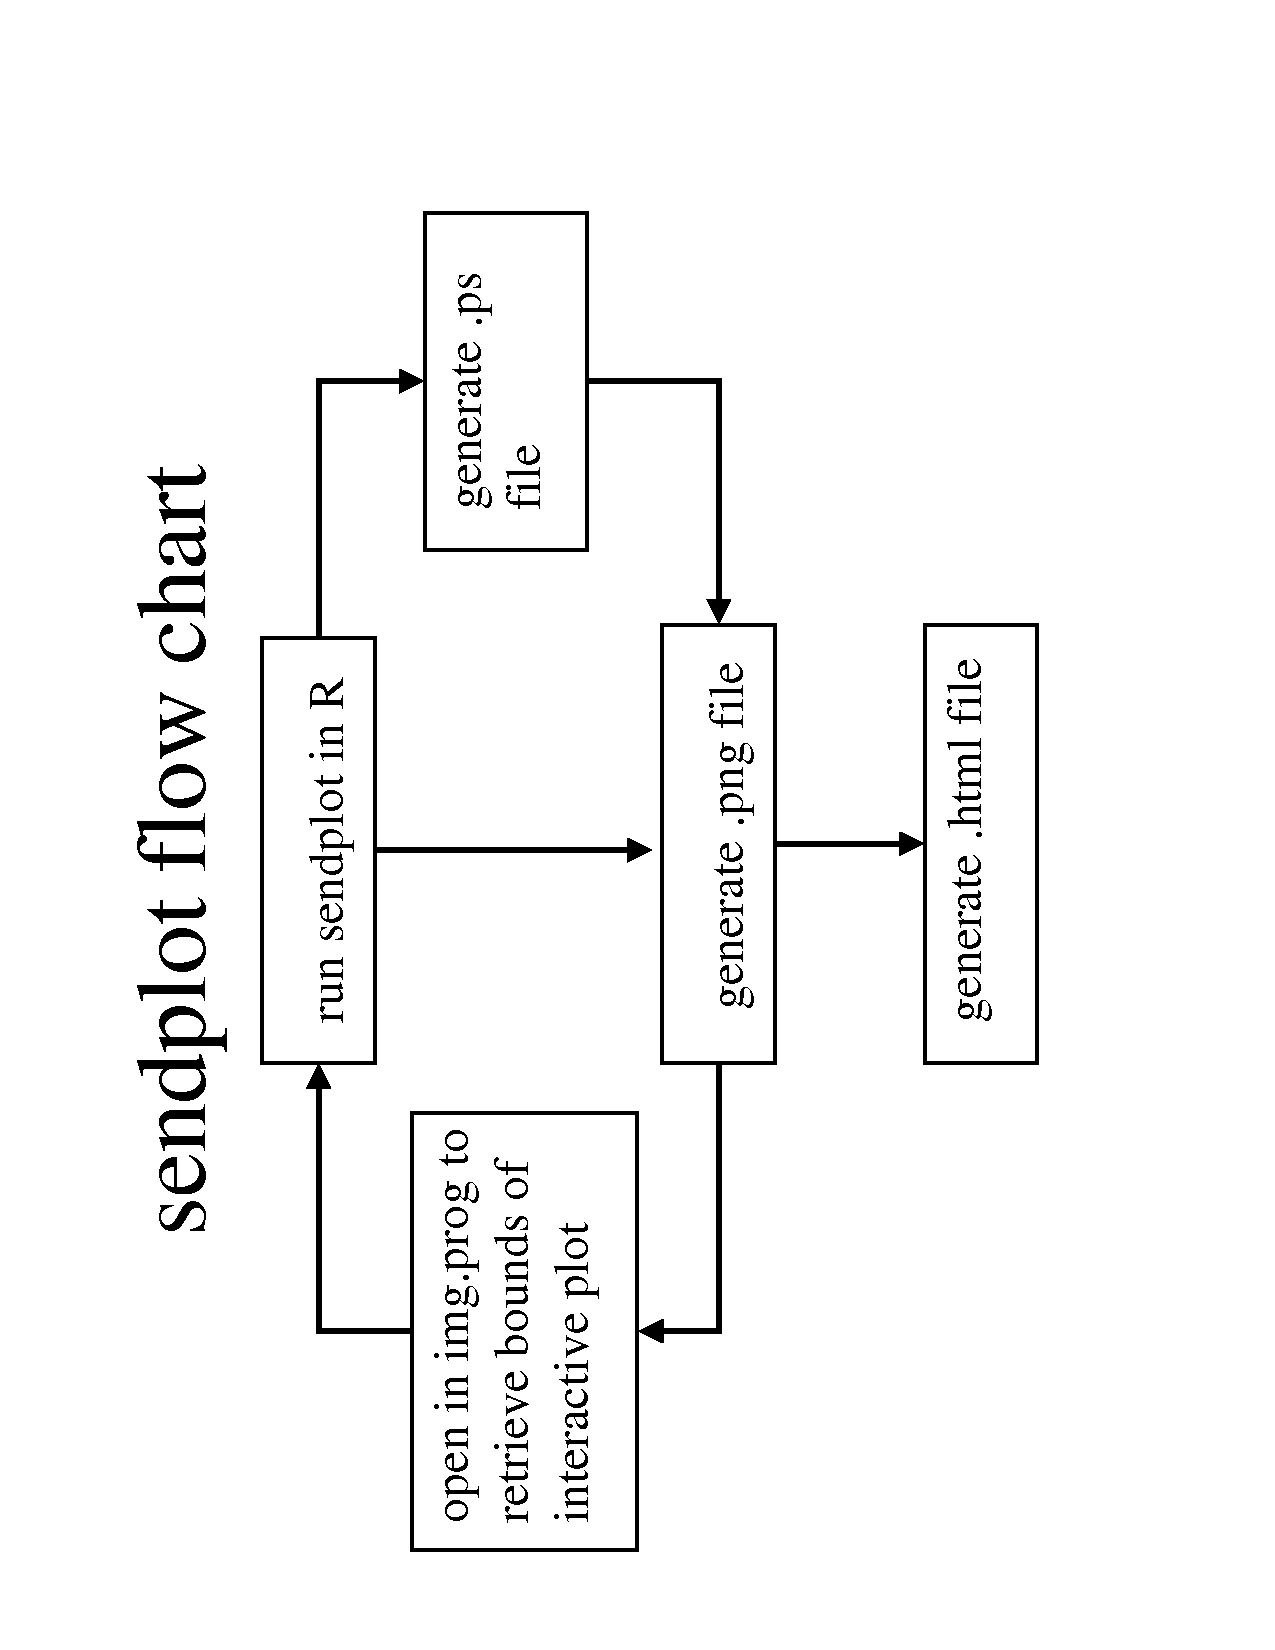
\includegraphics[angle=270]{sendplotFlowChart}
%\caption{The sendplot functions are typically run in two iterations when creating interactive plots for the first time. The first iteration involves the identification of the upper-left and lower-right pixel coordinates. The final output is generated in the second iteration.An option has bee implemented to eliminate this two step procedure for linux/unix machines.}
%\end{figure}
%\end{center}


\indent The remainder of this document will provide detailed tutorials for the use of the functions: xy.send, imagesend, heatmap.send, and the other main sendplot functions. All sections assume library has been loaded:

\begin{Schunk}
\begin{Sinput}
> library(sendplot)
\end{Sinput}
\end{Schunk}

\vskip5mm
\indent{\bf{Important Note:}} The sendplot output has been tested on Firefox and Internet Explorer browsers.  Internet Explorer users may need to modify their preferences to allow blocked content, as Internet Explorer may initially block the scripts from running. A warning message normally appears towards the top of the browser; if the user click on this warning it will give an option to allow blocked content.

%\newpage































\section{xy.send: scatter-plot wrapper}

The xy.send function creates a single interactive scatter-plot. The following is an example function call:
\begin{verbatim}
xy.send(plot.call, 
        x.pos,y.pos,
        plot.extras = NA,
        mai.mat=NA, mai.prc=FALSE,
        xy.labels=NA,
        image.size="800x1100",
        spot.radius = 5,
        fname.root="Splot",dir="./",
        window.size = "800x1100",...)
 \end{verbatim}

\subsection{specifying the plot call}
The plot.call argument is a character string containing the call for the desired scatter-plot. For example, consider the mtcars datasets provided to R users through the dataset package: the desired scatter-plot is gross horsepower vs miles per gallon.

\begin{center}
\begin{figure}
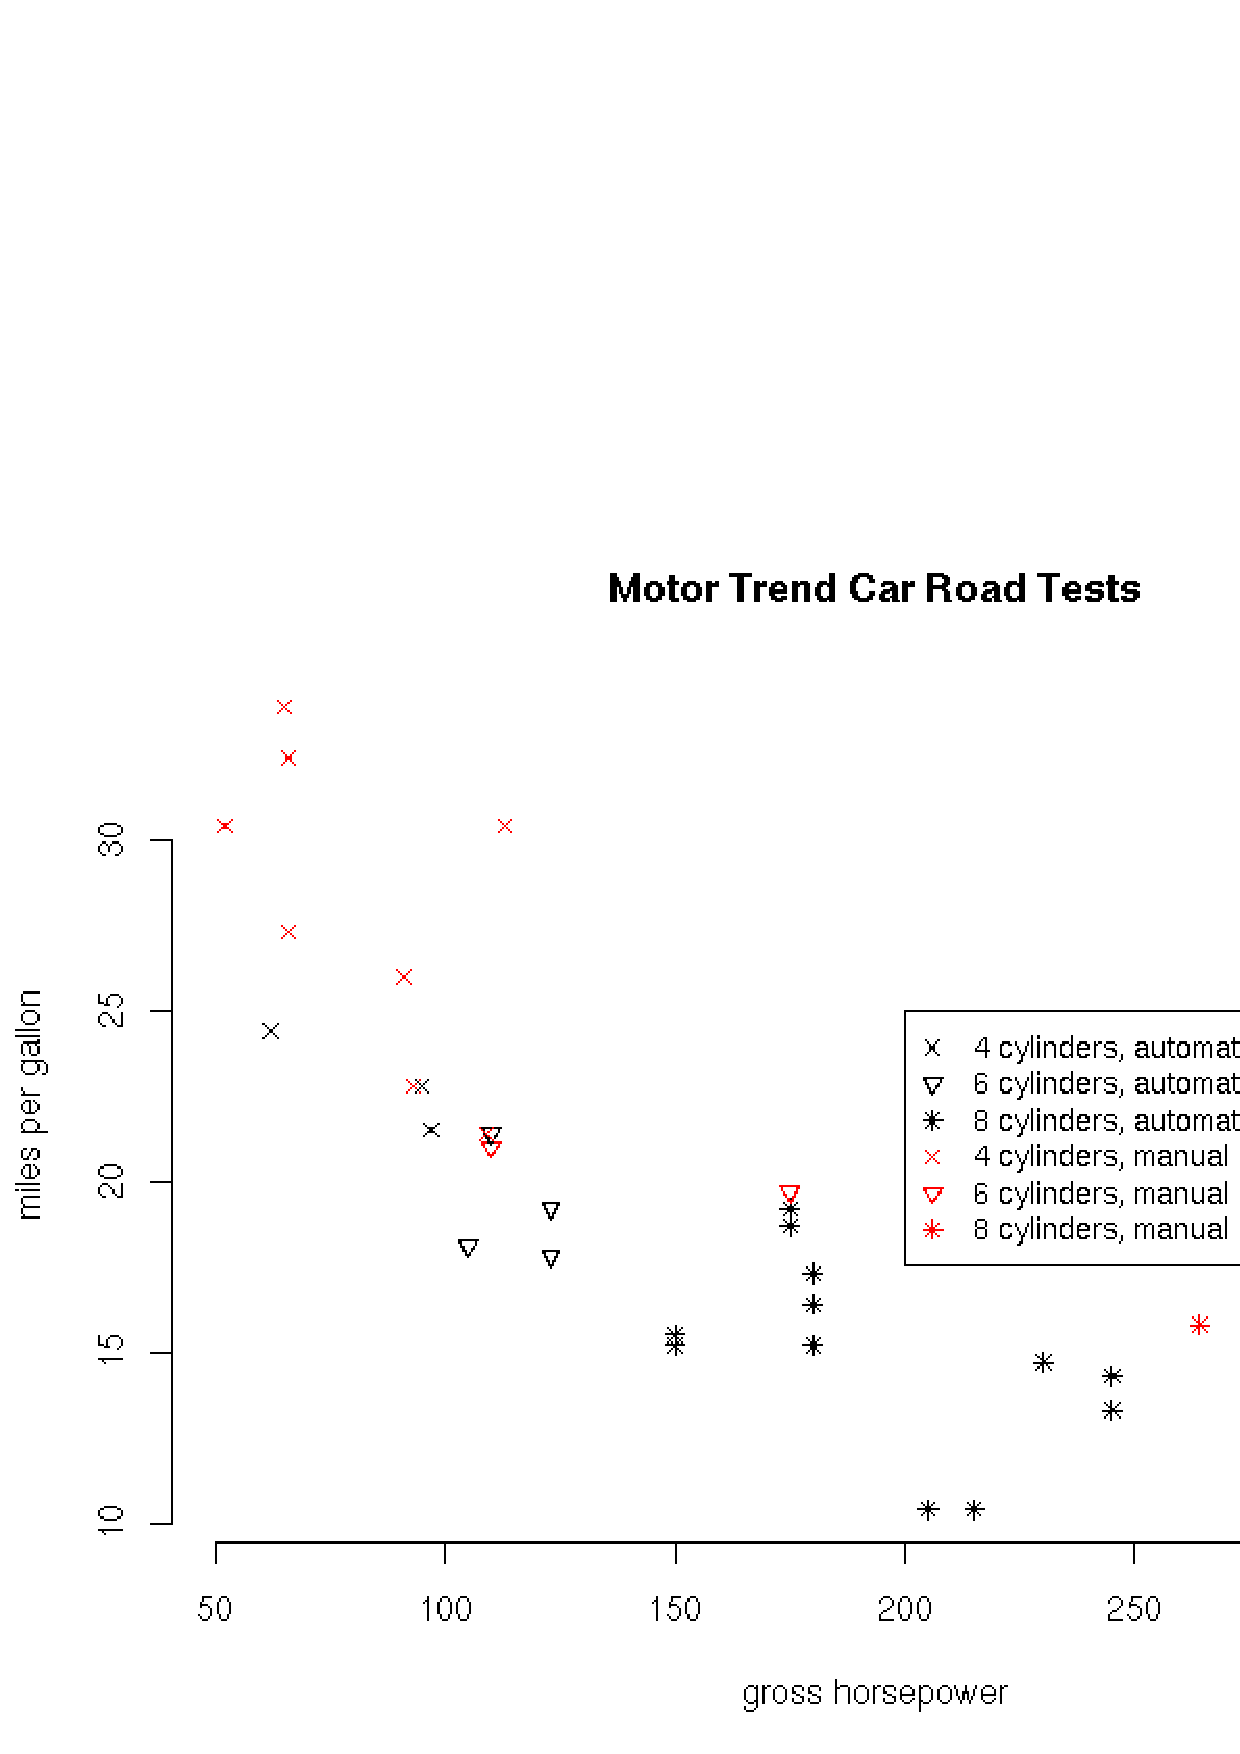
\includegraphics{exPlotXY}
\caption{scatter-plot using the mtcars dataset}
\end{figure}
\end{center}

The following example plot.call argument will generate the plot in figure 1. 

\begin{verbatim}
plot.call=c("plot(x.pos,y.pos,xlab='gross horsepower',
                   ylab='miles per gallon',axes=F,pch=mtcars$cyl,
                   col=mtcars$am+1,cex=0.875,
                   main='Motor Trend Car Road Tests');axis(1)")
\end{verbatim}


Notice that the call is a character string that will be evaluated as multiple function calls separated by a semicolon. Arguments of type character within these calls are specified with a single quotation rather than the double quotations used originally, or vice versa (see xlab argument). Any variables used in arguments (x.pos,y.pos in our example) should be in local memory before running the xy.send function call. \newline

\indent plot.extras is a list that contains additional expressions or plot calls. Each element of the list is a  character string to be evaluated as R functions. This can be used to add plotting features such as axes, legends, etc. \newline

The following adds an axis line and a legend to the example plot.


\begin{verbatim}
plot.extras=c("axis(2);
              legend(200,25,pch=rep(c(4,6,8),2),
                     col=c(rep(1,3),rep(2,3)),
                     legend=paste(rep(c(4,6,8),2),'cylinders,',
                     c('automatic','manual')[c(rep(1,3),rep(2,3))]),
              cex=0.875)")
\end{verbatim}

\indent Margins for the figure may be controlled through the mai.mat and mai.prc arguments. The mai.mat argument is a matrix n x 4 where n is the number of figures; for this wrapper mai.mat is a 1x4 matrix. The four columns represent the bottom, left, top, and right margins respectively. These values are passed into R's par(mai=) function. If mai.mat's values are a percentage of the original margins, mai.prc should be tripped to TRUE, if the values are values to be used for the margins then mai.prc is FALSE.


\subsection{specifying the interactive points, tool-tip content, and incorporating hyperlinks}

\indent The x.pos and y.pos arguments are the x and y coordinates of desired interactive points. This allows the user to decide if all points, a subset of points, or if any additional hidden/phantom points are interactive. In the example, all points will be interactive. 

\begin{verbatim}
y.pos=mtcars$mpg
x.pos=mtcars$hp
\end{verbatim}


\indent The argument xy.labels control what is displayed in the interactive window when the user hovers the mouse over plot points. 


\begin{verbatim}
xy.labels = data.frame(name=rownames(mtcars),mtcars=mtcars)
\end{verbatim}

\indent {\bf{Note:}} the function assumes the data.frame rows are in the same order as they appear in the x.pos (y.pos) argument. \newline
\\


\indent The additional arguments that may be passed into xy.send are any other parameters of the makeImap function. This includes asLinks and xy.links to add hyperlinks to tool-tip or to make the points themselves hyperlinks, as well as arguments for tool-tip display. See section 5.3 for more details on makeImap. 

\subsection{specifying the image.size and spot radius}

\indent The image.size determines the device width and height. \newline
\indent The spot.radius argument controls how large an area will be active when the mouse is scrolled over. If the user selects a larger region, some spot locations may overlap and be lost. The interactive application is very sensitive if the user selects a low region. The users' discretion is best used here given that the figure size, plot scale and number of data points will also play a role in determining a good spot.radius.  \\


\subsection{creating the xy.send example output}


\indent The xy.send function will use dir and fname.root to generate file names for the image (png or jpeg) and the html file. The following will create the files for the given example:


\begin{verbatim}

  xy.send(plot.call=plot.call,
       y.pos=y.pos,x.pos=x.pos,
       xy.labels = xy.labels, 
       plot.extras=plot.extras,
       image.size="800x600",
       fname.root="exPlotXY",
       font.size=18)
\end{verbatim}

\begin{center}
\begin{figure}
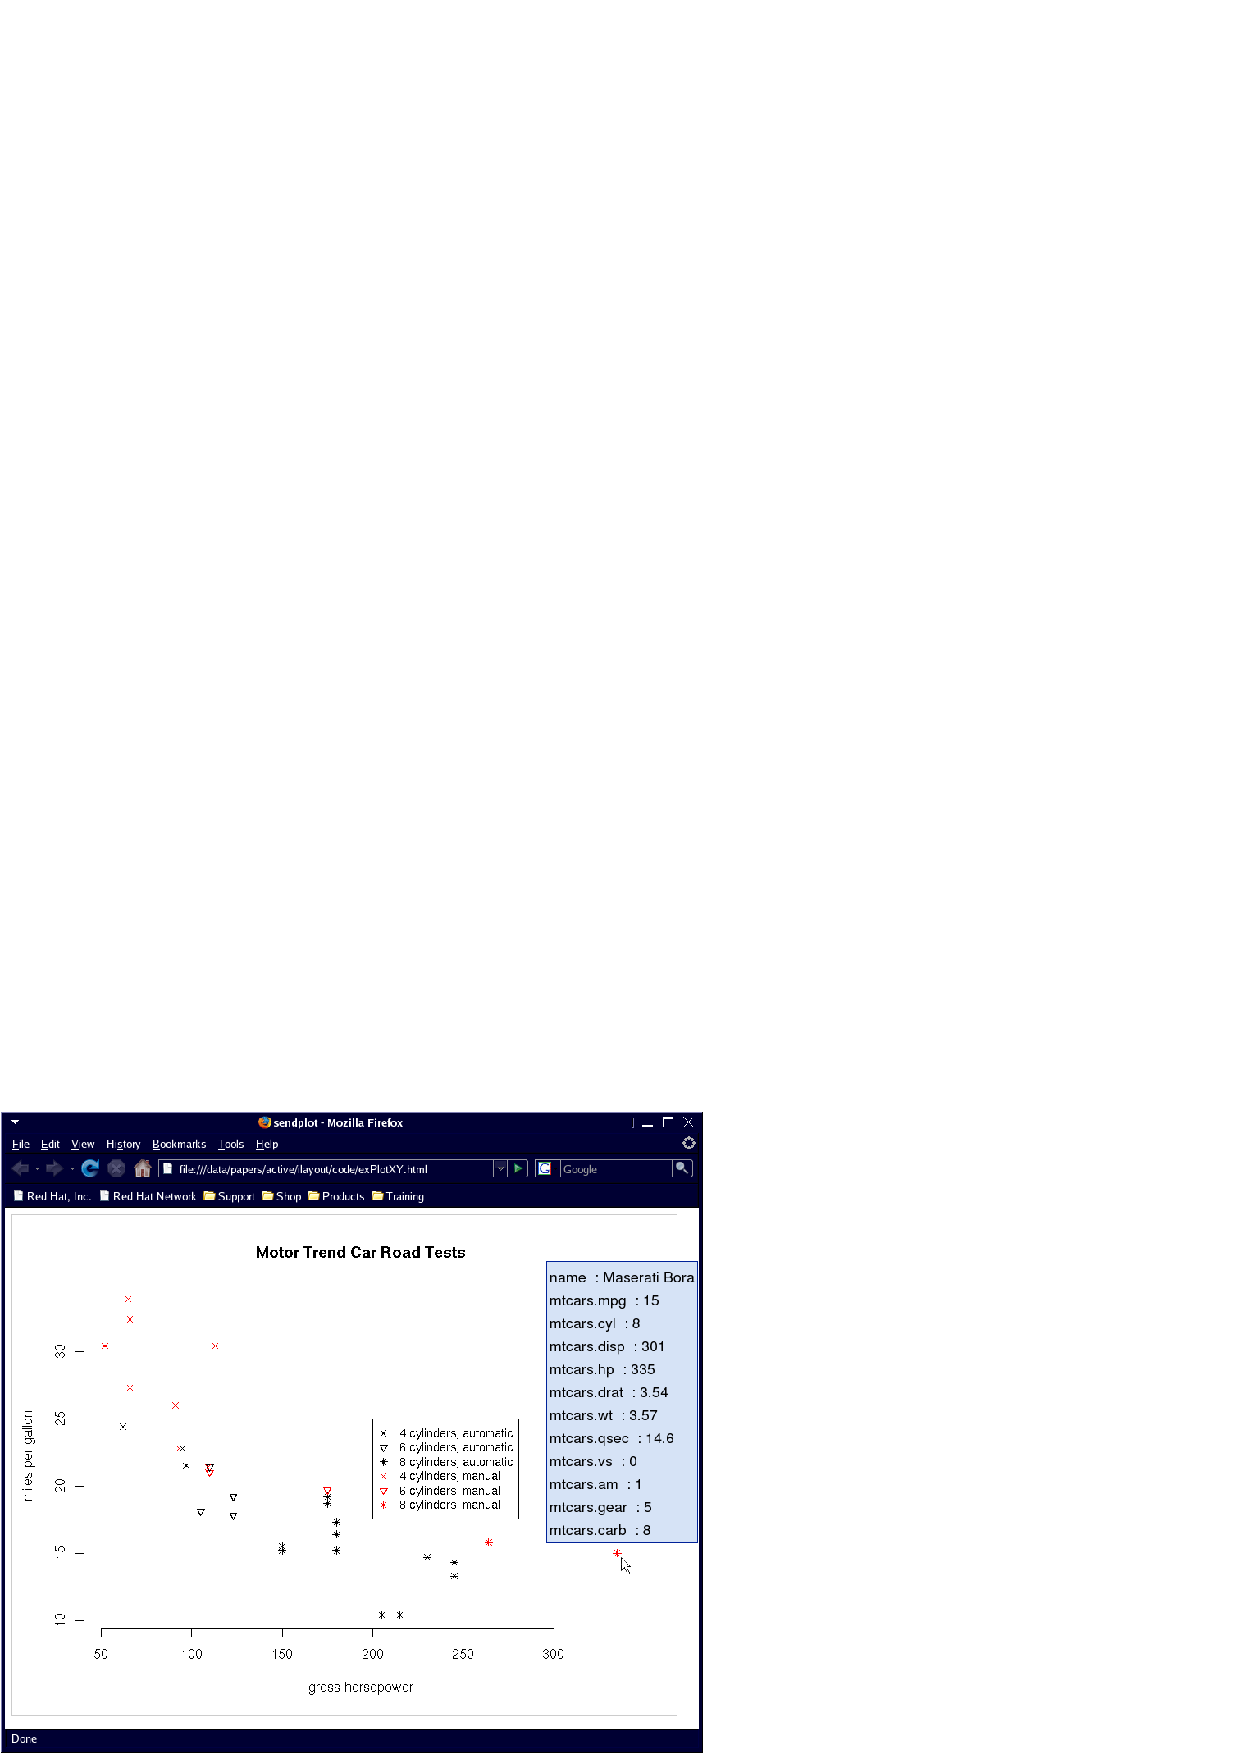
\includegraphics{iExPlotXY}
\caption{interactive scatter-plot using the mtcars dataset opened in Firefox web browser. Notice the tool-tip display box that appears for the specified point}
\end{figure}
\end{center}


\subsection{summary of code used to generate the sendxy example}

 The following is a summary of all code run to make the above example:

\begin{verbatim}
  library("sendplot")

  y.pos=mtcars$mpg
  x.pos=mtcars$hp

	 
  plot.call=c("plot(x.pos,y.pos,xlab='gross horsepower',
                   ylab='miles per gallon',axes=F,pch=mtcars$cyl,
                   col=mtcars$am+1,cex=0.875,
                   main='Motor Trend Car Road Tests');axis(1)")


  plot.extras=c("axis(2);
              legend(200,25,pch=rep(c(4,6,8),2),
                     col=c(rep(1,3),rep(2,3)),
                     legend=paste(rep(c(4,6,8),2),'cylinders,',
                     c('automatic','manual')[c(rep(1,3),rep(2,3))]),
              cex=0.875)")

  xy.labels = data.frame(name=rownames(mtcars),mtcars=mtcars)


 
  xy.send(plot.call=plot.call,
       y.pos=y.pos,x.pos=x.pos,
       xy.labels = xy.labels, 
       plot.extras=plot.extras,
       image.size="800x600",
       fname.root="exPlotXY",
       font.size=18)

\end{verbatim}


And there you have it, an interactive scatter-plot! 

\newpage




























\section{imagesend: image wrapper}

The imagesend function creates a single interactive image. The following is an example function call: 

\begin{verbatim}
imagesend(plot.call, 
           x.pos, y.pos,
           xy.type,
           plot.extras = NA,
           mai.mat=NA, mai.prc=FALSE,
           xy.labels=NA,
           image.size="800x1100",
           spot.radius = 5,
           fname.root="Splot",
           dir="./",
           window.size = "800x1100",...)


\end{verbatim}

For the most part the arguments for imagesend are consistent with those for xy.send. 

\subsection{specifying the plot call}
As with the xy.send function, the plot.call argument is a character string containing the call for the desired image plot. Consider the following example data from the mtcars dataset:
\begin{verbatim}

carsX  = as.matrix(mtcars)
carsX <- sweep(carsX, 2, colMeans(carsX, na.rm = T))
        sx <- apply(carsX, 2, sd, na.rm = T)
        carsX <- sweep(carsX, 2, sx, "/")

x = 1:dim(carsX)[2]
y = 1:dim(carsX)[1]
z = t(carsX)
\end{verbatim}



\begin{center}
\begin{figure}
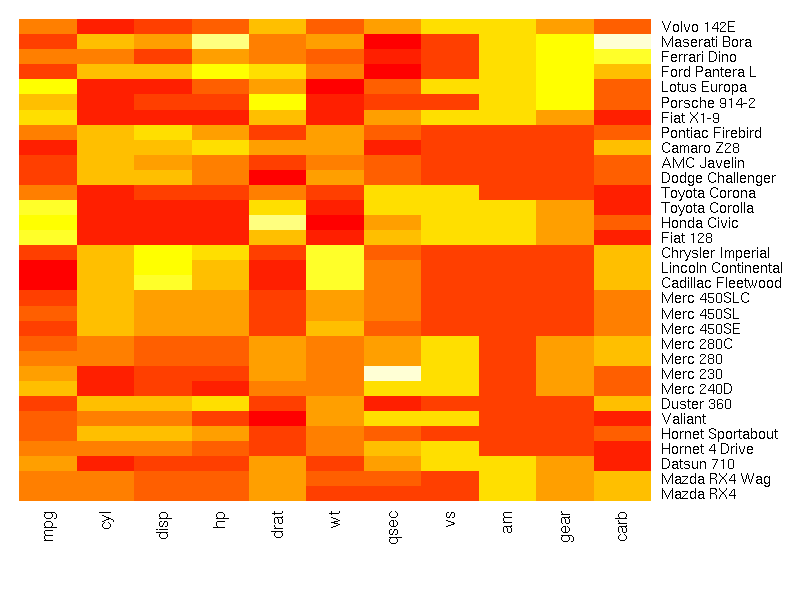
\includegraphics{exPlotImage}
\caption{heatmap image using the mtcars dataset}
\end{figure}
\end{center}

The following constructs a plot.call argument for figure 3. 

\begin{verbatim}

plot.call = "image(x=x,y=y, z=z,
                    axes = FALSE, xlab = '', ylab = '');
              axis(1,1:dim(carsX)[2], 
                   labels=colnames(carsX),
                   las = 2, line = -0.5, tick = 0,cex.axis =1); 
              axis(4,1:dim(carsX)[1], 
                   labels=rownames(carsX),
                   las = 2, line = -0.5, tick = 0,cex.axis =.8)"

\end{verbatim}


Notice how the call is a character string that will be evaluated as multiple function calls separated by a semicolon.  Arguments of type character within these calls are specified with a single quotation rather than the double quotations used originally, or vice versa. Any variables used in arguments (x,y,z in our example) should be in local memory before running the imagesend function call. \newline

\indent The mai.mat and mai.prc arguments function the same as in the xy.send function; see section 2.1.  The following sets the margins for the image. 

\begin{verbatim}
mai.mat = matrix(c(1,.2,.2,1.5), ncol=4)
mai.prc = FALSE
\end{verbatim}


\subsection{specifying the interactive points, tool-tip content, and hyperlinks}

\indent The x.pos and y.pos arguments are the x and y values to be used for interactive regions; generally these will be the same as the x and y arguments of the image call. x and y may be the locations of the grid lines at which the values of z correspond or the midpoints of the regions of the image. xy.type will determine how x.pos and y.pos are treated: options include image.midpoint, image.boundaries, and image.box among others. For complete listing of xy.type options see section 5.3. The additional arguments in the imagesend function call refer to any other arguments to be passed into the makeImap function; see section 5.3 for more details. This includes but is not limited to the x.labels, y.labels, xy.links, y.link, x.links, and arguments for controlling the tool-tip window display.

\indent As with the xy.send function, the arguments x.labels, y.labels, and xy.labels control what is displayed in the interactive window when the user hovers the mouse over designated points. The arguments x.labels and y.labels refer to data that is specific to the x and y values respectively. x.labels and y.labels are data.frames of the dimension n by m, where n is equal to the length of x or y respectively. Each row is specific to a certain x or y value and each column is a unique variable or characteristic of x or y respectively.  The first row of the data frames should contain column headers; these names will be used as display names in the interactive window that appears. The xy.labels argument is a little different because it governs data specific to both x and y locations. The function argument xy.labels is a list of matrices; each matrix is of the dimension n by m, where n is equal to the length of y and m is equal to the length of x.\\ 

\indent Consider the mtcars example dataset:

\begin{verbatim}
xy.labels=list(value=round(carsX,3))

x.labels=data.frame(
       label=colnames(carsX),
       description=c("Miles/(US) gallon",
                     "Number of cylinders",
                     "Displacement (cu.in.)",
                     "Gross horsepower",
                     "Rear axle ratio",
                     "Weight (lb/1000)",
                     "1/4 mile time",
                     "V/S",
                     "Transmission (0 = automatic, 1 = manual)",
                     "Number of forward gears",
                     "Number of carburetors")
       )

\end{verbatim}


\indent {\bf{Note:}} The function assumes the data.frame rows are in the same order as they appear in the x.pos argument (or y.pos argument if y.labels).  \newline

\indent As with the xy.send function, any of the hyperlink may be included through the asLinks, x.links, y.links, or xy.links arguments. The x.link, y.links and xy.links behave the same as x.labels, y.labels, and xy.labels respectively; they however, contain complete web addresses as character strings. For an image, asLinks has several acceptable forms. It may be a matrix or data frame of the dimensions n by m, where n is equal to the length of y and m is equal to the length of x. asLinks may also be a vector of length equal to length of x times length of y, thus a vector version of the fore-mentioned matrix or data frame. These options may be useful when xy specific hyperlinks are desired (similar to an xy.lbls argument). asLinks may also be a vector of length equal to the length of x or y, indicating x, or y, specific hyperlinks. If asLinks is of length x, the vector will be repeated length of y so that every similar x value will be the same hyperlink, and vice versa for y. If asLinks is of length one and is not NA, the value will be repeated for every grid location. NA represent a point that is not a hyperlink.  Every asLink entry should be a character string for a complete web address or NA. Additional arguments for the makeImap function may be utilized. For more information and examples see section 5.3

\subsection{specifying the image.size and spot radius}

\indent The image.size and spot.radius argument for imagesend are the same as in xy.send. Please refer to section 2.3. 


\subsection{creating the imagesend example output}


\indent The imagesend function will use dir and fname.root to generate file names for the image (png or jpeg) and the html file. The following will create the files for the given example:


\begin{verbatim}

  imagesend(plot.call=plot.call,
       y.pos=y,x.pos=x,
       mai.mat=mai.mat, mai.prc=mai.prc,
       xy.type="image.midpoints",
       x.labels=x.labels,
       xy.labels = xy.labels, 
       image.size="800x600",
       fname.root="exPlotImage", 
       font.size=18)

\end{verbatim}


\begin{center}
\begin{figure}
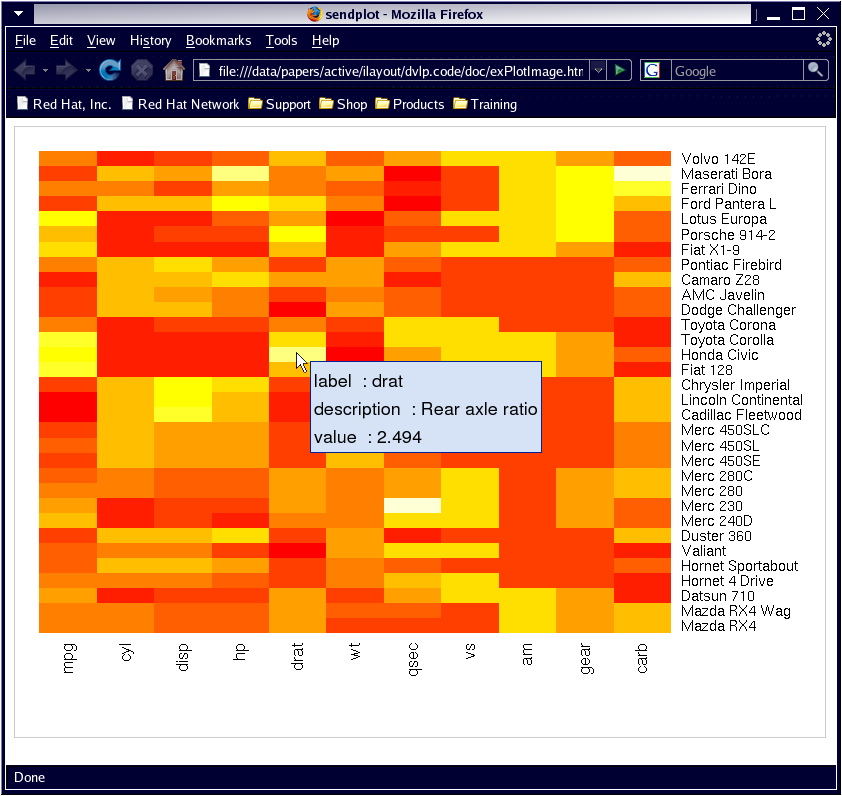
\includegraphics{iExPlotImage}
\caption{interactive heatmap image using the mtcars dataset, viewed using the Firefox web browser. Notice the tool-tip displayed for the identified region.}
\end{figure}
\end{center}


\subsection{summary of code used to generate imagesend example}

 The following is a summary of all code run to make the above example:

\begin{verbatim}
 library("sendplot")

carsX  = as.matrix(mtcars)
carsX <- sweep(carsX, 2, colMeans(carsX, na.rm = T))
        sx <- apply(carsX, 2, sd, na.rm = T)
        carsX <- sweep(carsX, 2, sx, "/")

x = 1:dim(carsX)[2] ; y = 1:dim(carsX)[1] ; z = t(carsX)

plot.call = "image(x=x,y=y, z=z,
                    axes = FALSE, xlab = '', ylab = '');
              axis(1,1:dim(carsX)[2], 
                   labels=colnames(carsX),
                   las = 2, line = -0.5, tick = 0,cex.axis =1); 
              axis(4,1:dim(carsX)[1], 
                   labels=rownames(carsX),
                   las = 2, line = -0.5, tick = 0,cex.axis =.8)"

mai.mat = matrix(c(1,.2,.2,1.5), ncol=4)
mai.prc = FALSE

xy.labels=list(value=round(carsX,3))

x.labels=data.frame(
       label=colnames(carsX),
       description=c("Miles/(US) gallon","Number of cylinders",
                     "Displacement (cu.in.)",
                     "Gross horsepower",
                     "Rear axle ratio",
                     "Weight (lb/1000)",
                     "1/4 mile time",
                     "V/S",
                     "Transmission (0 = automatic, 1 = manual)",
                     "Number of forward gears",
                     "Number of carburetors")
       )

imagesend(plot.call=plot.call,
       y.pos=y,x.pos=x,
       mai.mat=mai.mat, mai.prc=mai.prc,
       xy.type="image.midpoints",
       x.labels=x.labels,
       xy.labels = xy.labels, 
       image.size="800x600",
       fname.root="exPlotImage",
       font.size=18)
\end{verbatim}
And there you have it, an interactive image! 
\newpage




























\section{heatmap.send: heatmap wrapper}


The heatmap.send function creates a interactive heatmap image in the style of the R stats package heatmap function. This is a wrapper connecting the heatmap function of the R stats package with sendplot. The majority of the code for this function is verbatim from the R package stats heatmap function. This function was designed to work as a wrapper to utilize the same functionality and plotting as the heatmap function with sendplot's interactive functionality. Authors of heatmap code used in our code: Andy Liaw, original; R. Gentleman, M. Maechler, W. Huber,revisions. The following is an example function call: 


\begin{verbatim}

heatmap.send(x,
             Rowv = NULL,
             Colv = if (symm) "Rowv" else NULL, 
             distfun = dist,
             hclustfun = hclust,
             reorderfun = function(d,w) reorder(d, w),
             add.expr,
             symm = FALSE,
             revC = identical(Colv,"Rowv"),
             scale = c("row", "column", "none"),
             na.rm = TRUE, 
             margins = c(5, 5),
             ColSideColors,
             RowSideColors,
             cexRow = 0.2 +  1/log10(nr),
             cexCol = 0.2 + 1/log10(nc),
             labRow = NULL, 
             labCol = NULL,
             main = NULL,
             xlab = NULL,
             ylab = NULL,
             keep.dendro = FALSE, 
             verbose = getOption("verbose"),
             x.labels=NA,y.labels=NA,
             xy.labels=NA,x.links=NA,
             y.links=NA,xy.links=NA,
             asLinks=NA,
             spot.radius=5,
             source.plot=NA,
             image.size="800x1100",
             fname.root="test",dir="./",
             header="v2",window.size = "800x1100", 
             ...) 
\end{verbatim}


\indent {\bf{Note:}} Most of the arguments in this function are arguments for the stats package function heatmap. The reader is referred to heatmap documentation for additional information regarding arguments which are common to both functions.. \newline



\subsection{specifying the plot call}

The function heatmap.send differs from the previous functions, xy.send and imagesend, in that there is no plot.call argument. The heatmap function in the R stats package takes in a matrix of values, x,  and makes a corresponding image. The mtcars example from the datasets package will be use to create figure 5:  

\begin{verbatim}
x  = as.matrix(mtcars)
\end{verbatim}


\begin{center}
\begin{figure}
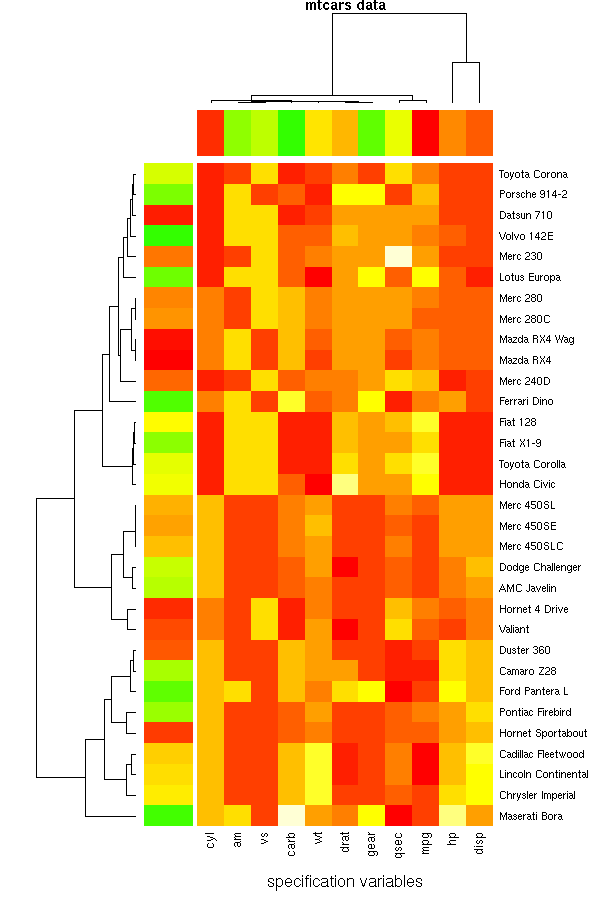
\includegraphics{exHeat}
\caption{heatmap image using the mtcars dataset utilizing R's heatmap function}
\end{figure}
\end{center}

\subsection{specifying the interactive points,tool-tip content, and hyperlinks}


\indent As with the xy.send function, the arguments x.labels, y.labels, and xy.labels control what is displayed in the interactive window when the user hovers the mouse over plot points. The arguments x.labels and y.labels refer to data that is specific to the x and y values respectively. x.labels and y.labels are data.frames. x.labels is of the dimension n by m where n is equal to the width of the argument x. y.labels is of the dimension n by m where n is equal to the length of the argument x. Each row is specific to a certain x or y value and each column is a unique variable or characteristic of x or y respectively.  The first row of the data frames should contain column headers; these names will be used as display names in the interactive window that appears. xy.labels refers to data that is specific to both x and y location. The function argument xy.labels is a list of matrices; each matrix should be of the same dimensions as x.

\begin{verbatim}
xy.labels=list(value=x)

x.labels=data.frame(
      label=colnames(x),
      description=c("Miles/(US) gallon","Number of cylinders",
                    "Displacement (cu.in.)",
                    "Gross horsepower",
                    "Rear axle ratio",
                    "Weight (lb/1000)",
                    "1/4 mile time",
                    "V/S",
                    "Transmission (0 = automatic, 1 = manual)",
                    "Number of forward gears",
                    "Number of carburetors")
      ) 

\end{verbatim}


\indent {\bf{Note:}} The function assumes the data.frame rows are in the same order as they appear in the x argument.  \newline

\indent As with the send.image function, asLinks is used to make grid locations hyperlinks. Also, the arguments x.links, y.links, and xy.links are used to display hyperlinks in the interactive window. Other additional arguments for the makeImap function may be utilized. Please refer to section 5.3.


\indent The heatmap function allows for a few different options including color-coded bars for x and y samples, as well as clustering. The following code creates a schema of colors for samples. 
\begin{verbatim}
# color bars for samples
rc = rainbow(nrow(x), start=0, end=.3)
cc = rainbow(ncol(x), start=0, end=.3)
\end{verbatim}


\subsection{specifying the image.size and spot radius}

\indent The image.size and spot.radius argument for heatmap.send are the same as in xy.send. Please refer to section 2.3.

\subsection{creating the heatmap.send example output}

\indent The heatmap.send function will use dir and fname.root to generate file names for the image (png or jpeg) and the html file. The following will create the files for the given example:




\begin{verbatim}

 heatmap.send(x, scale="column",
              xy.labels = xy.labels,
              x.labels=x.labels,
              RowSideColors = rc,
              ColSideColors = cc, 
              margin=c(5,10),
              xlab = "specification variables", 
              ylab= "Car Models",
              main = "mtcars data",
              fname.root="exHeat", 
              font.size=18,image.size="600x900")

\end{verbatim}

\begin{center}
\begin{figure}
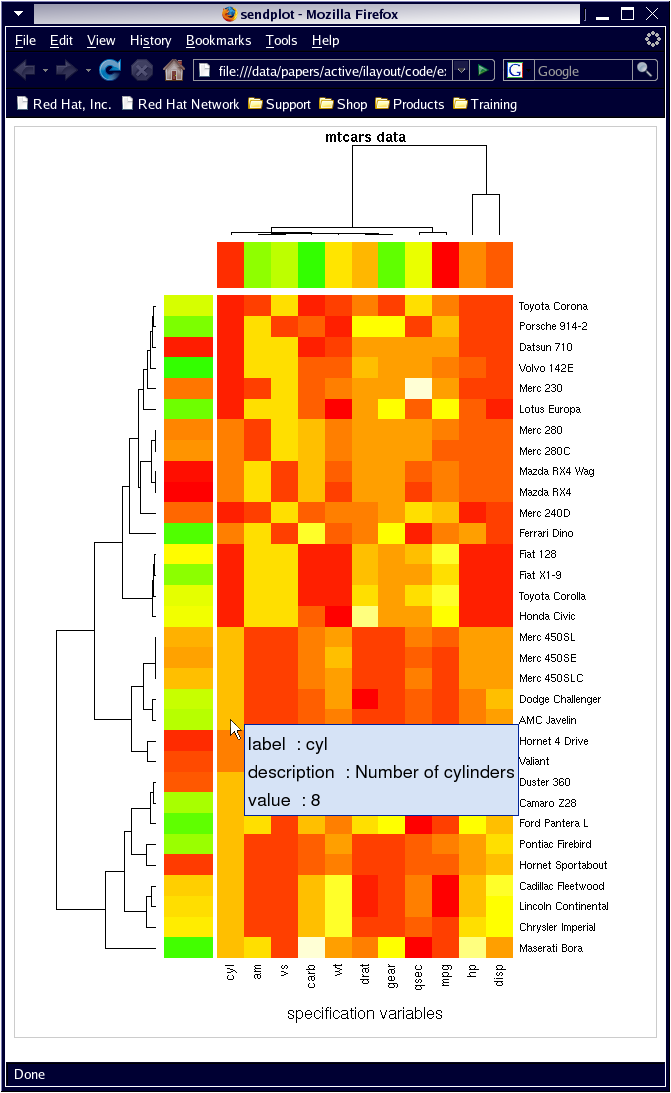
\includegraphics{iExHeat}
\caption{interactive heatmap image using the mtcars dataset utilizing R's heatmap function. Notice the tool-tip displayed for the identified region }
\end{figure}
\end{center}

\subsection{summary of code used to generate the heatmap.send example}

 
The following is a summary of all code run to make the above example:

\begin{verbatim}
library("sendplot")

x  = as.matrix(mtcars)
rc = rainbow(nrow(x), start=0, end=.3)
cc = rainbow(ncol(x), start=0, end=.3)

xy.labels=list(value=x)

x.labels=data.frame(
       label=colnames(x),
       description=c("Miles/(US) gallon","Number of cylinders",
                     "Displacement (cu.in.)",
                     "Gross horsepower",
                     "Rear axle ratio",
                     "Weight (lb/1000)",
                     "1/4 mile time",
                     "V/S",
                     "Transmission (0 = automatic, 1 = manual)",
                     "Number of forward gears",
                     "Number of carburetors")
       ) 


 heatmap.send(x, scale="column",
              xy.labels = xy.labels,
              x.labels=x.labels,
              RowSideColors = rc,
              ColSideColors = cc, 
              margin=c(5,10),
              xlab = "specification variables", 
              ylab= "Car Models",
              main = "mtcars data",
              fname.root="exHeat", 
              font.size=18,image.size="600x900")


\end{verbatim}


And there you have it, an interactive heatmap! 


\newpage





























\section{Interactive Layout of Plots}

\indent There are three main functions for creating an interactive layout of plots. These functions are:

\begin{description}
\item{initSplot:~}{initializes a 'splot' object}
\item{makeImap:~}{adds tool-tip data to 'splot' object}
\item{makeSplot:~}{uses 'splot' object to create static display and interactive HTML}
\end{description}

\indent This section will look at each of these functions in more detail as well as two other functions: addDefault and removeImap. 


\subsection{initSplot: Initializing the 'Splot' Object}

\indent The initSplot function creates a sendplot 'Splot' object. This object holds all information needed to generate a static layout of plots.  The following  is an example function call:

\begin{verbatim}

initSplot(mat,
         plot.calls,
         Iflag=NA, figTypes=NA,
         mai.mat=NA, mai.prc=FALSE,
         plot.extras = NA,
         source.plot=NA,image.size="800x1100",
         pointsize=12, res=NA,
         ps.paper="letter",ps.width=8,ps.height=11,
         returnVl=T,
         saveFlag=F,saveName="Splot.RData")

\end{verbatim}


We provide the code below to generate the interactive plot displayed in Figure 7. The plot is does not constitute a practical use example, rather it serves to illustrates many of the capabilities sendplot has to offer.  \newline

\newpage
\begin{center}
\begin{figure}
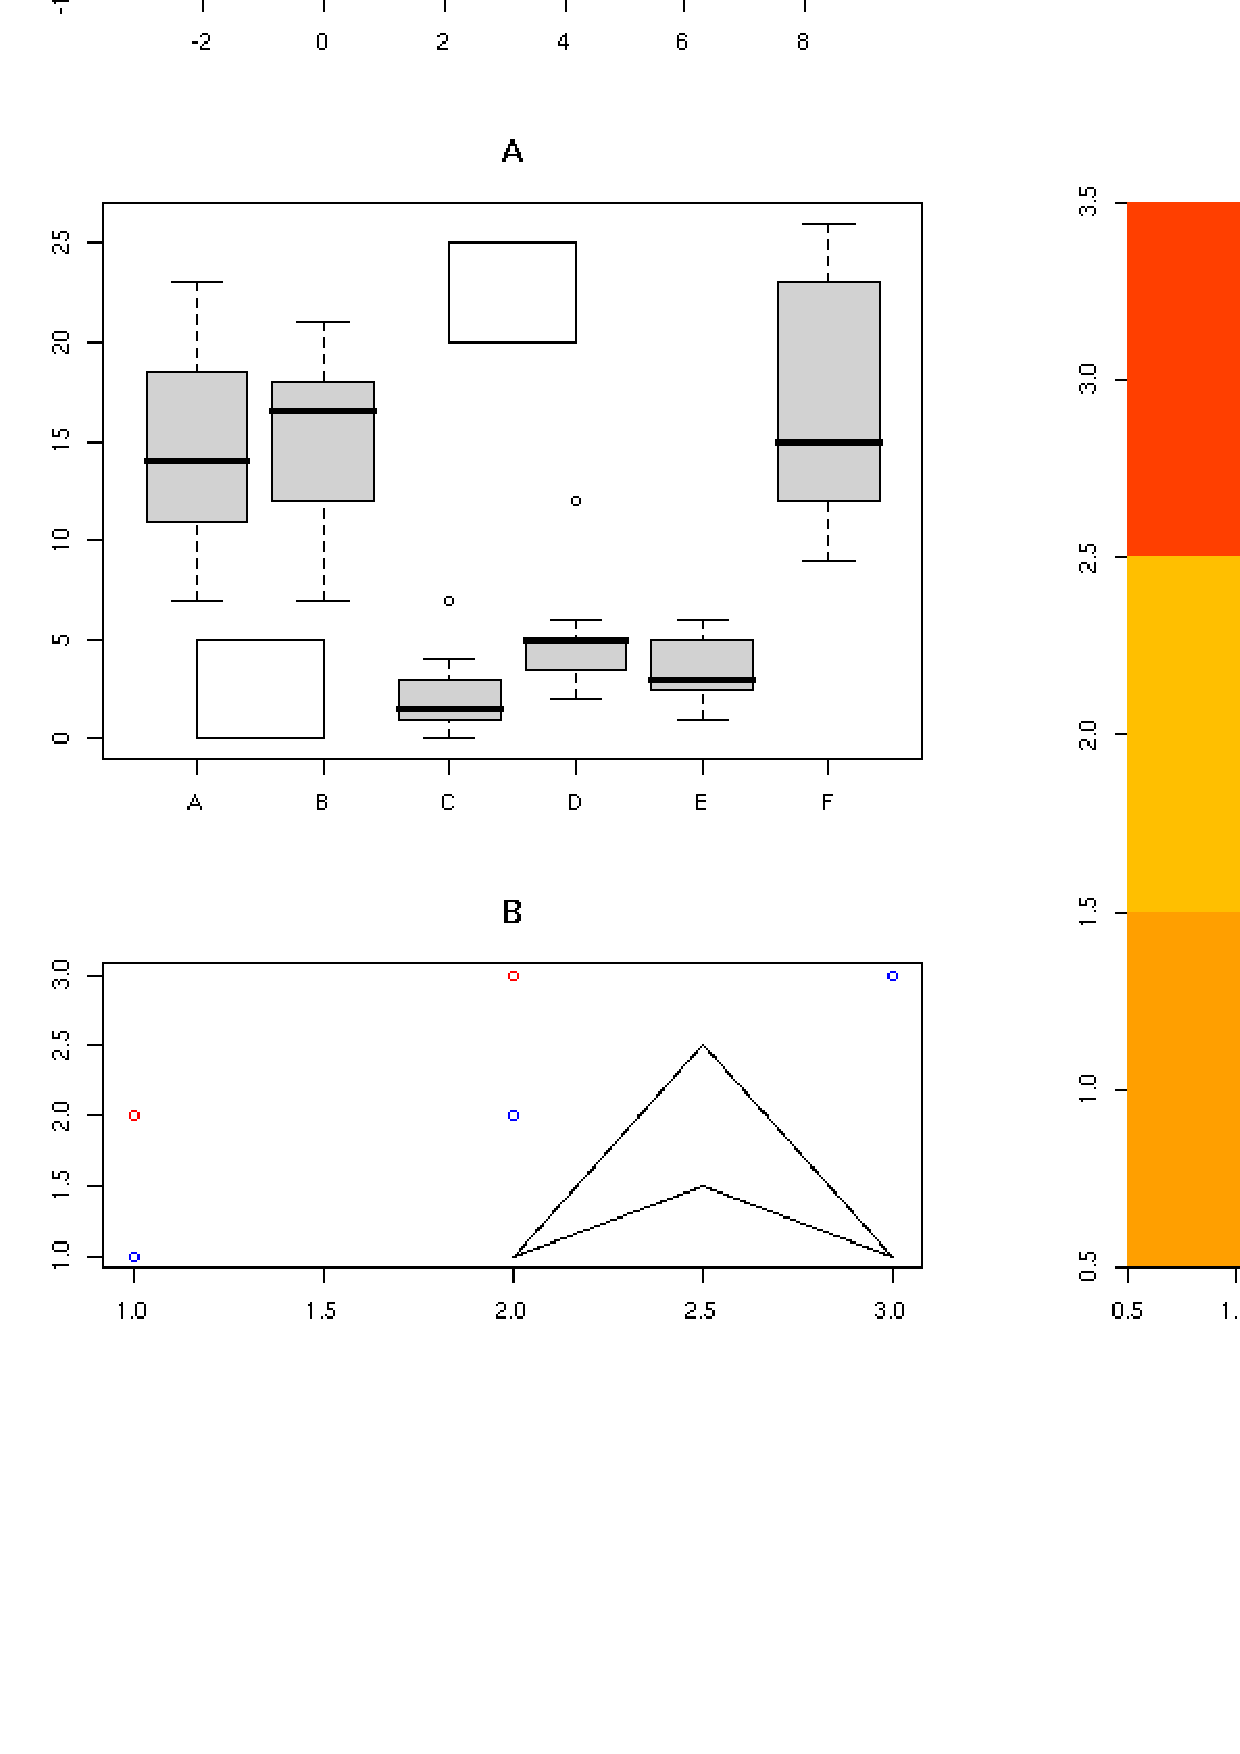
\includegraphics{FirstLookEx}
\caption{Layout of multiple figures}
\end{figure}
\end{center}

\subsubsection{specifying the plot call}

This section will define the following initSplot arguments:

\begin{description}
   \item{mat:~}{numeric matrix governing plot layout}
   \item{plot.calls:~}{character vector of desired plot calls}
   \item{Iflag:~}{numeric vector indicating which plots have interactive data}
   \item{figTypes:~}{character vector of the figures' plot type E.g. 'scatterplot','image','heatmap','tiling'}
   \item{mai.mat:~}{numeric matrix indicating plot margins}
   \item{mai.prc:~}{logical indicating if mai.mat is a percentage of default settings}
   \item{plt.extras:~}{character vector of additional plotting}
\end{description}

\indent The first argument of initSplot, mat, is a numeric matrix that is passed into the R graphics package function layout. The example will be a layout with four figures. 

\begin{verbatim}
mat = matrix(c(rep(c(rep(4,8),rep(0,5)),2),
               rep(c(rep(1,8),rep(3,5)),6),
               rep(c(rep(2,8),rep(3,5)),4)),
               byrow=T, ncol=13)

\end{verbatim}

\indent This results in the following matrix:

\begin{Schunk}
\begin{Soutput}
      [,1] [,2] [,3] [,4] [,5] [,6] [,7] [,8] [,9] [,10] [,11] [,12] [,13]
 [1,]    4    4    4    4    4    4    4    4    0     0     0     0     0
 [2,]    4    4    4    4    4    4    4    4    0     0     0     0     0
 [3,]    1    1    1    1    1    1    1    1    3     3     3     3     3
 [4,]    1    1    1    1    1    1    1    1    3     3     3     3     3
 [5,]    1    1    1    1    1    1    1    1    3     3     3     3     3
 [6,]    1    1    1    1    1    1    1    1    3     3     3     3     3
 [7,]    1    1    1    1    1    1    1    1    3     3     3     3     3
 [8,]    1    1    1    1    1    1    1    1    3     3     3     3     3
 [9,]    2    2    2    2    2    2    2    2    3     3     3     3     3
[10,]    2    2    2    2    2    2    2    2    3     3     3     3     3
[11,]    2    2    2    2    2    2    2    2    3     3     3     3     3
[12,]    2    2    2    2    2    2    2    2    3     3     3     3     3
\end{Soutput}
\end{Schunk}

\indent {\bf{Note:}} In layout, zero acts as a region in which no graph is displayed, a buffer. Notice the use of zero to allow the width of the first and fourth plot to line up in the example.
\vskip 10mm


\indent Figure 8 displays a box version of the above layout.
\begin{center}
\begin{figure}

\includegraphics{LayoutFig}
\caption{box display of layout}
\end{figure}
\end{center}


\indent The plot.calls argument is a character vector containing the desired plot calls for all graphs. The order of the plot.calls should correspond to the desired plotting region in the layout. The plot calls argument for the example is of length four:


\begin{verbatim}

plot.calls = c(
    "boxplot(count ~ spray, data = InsectSprays, col = 'lightgray')",

    "plot(1:3,1:3, col='blue', xlab='', ylab=''); points(1:2, 2:3, col='red')", 

    "image(1:2,1:3, z=matrix(myX,ncol=3,nrow=2), xlab='', ylab='')",

    "plot(cos, xlim = c(-pi,3*pi), n = 1001, col = 'blue', xlab='', ylab='')" )


\end{verbatim}


\indent The first plot call (given figure 9) creates a boxplot that looks like:

\begin{verbatim}
boxplot(count ~ spray, data = InsectSprays, col = 'lightgray')
\end{verbatim}



\begin{center}
\begin{figure}
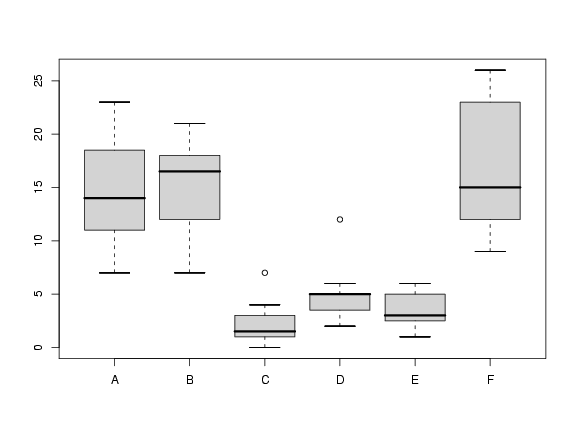
\includegraphics{boxplot}
\caption{plot 1 of the layout is a boxplot}
\end{figure}
\end{center}

\indent The second plot call (given figure 10) creates a scatterplot of three blue points in a diagonal and two red points in a parallel diagonal. 

\begin{verbatim}
plot(1:3,1:3, col='blue', xlab='', ylab=''); points(1:2, 2:3, col='red')
\end{verbatim}

\begin{center}
\begin{figure}
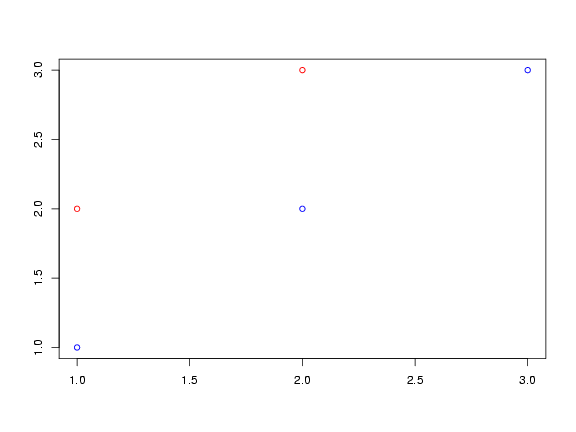
\includegraphics{scatter}
\caption{plot 2 of the layout is a scatterplot}
\end{figure}
\end{center}

\indent The third plot call, given by:
\begin{verbatim}
image(1:2,1:3, z=matrix(myX,ncol=3,nrow=2), xlab='', ylab='')
\end{verbatim}
creates a 2x3 image seen in figure 11.


\begin{center}
\begin{figure}
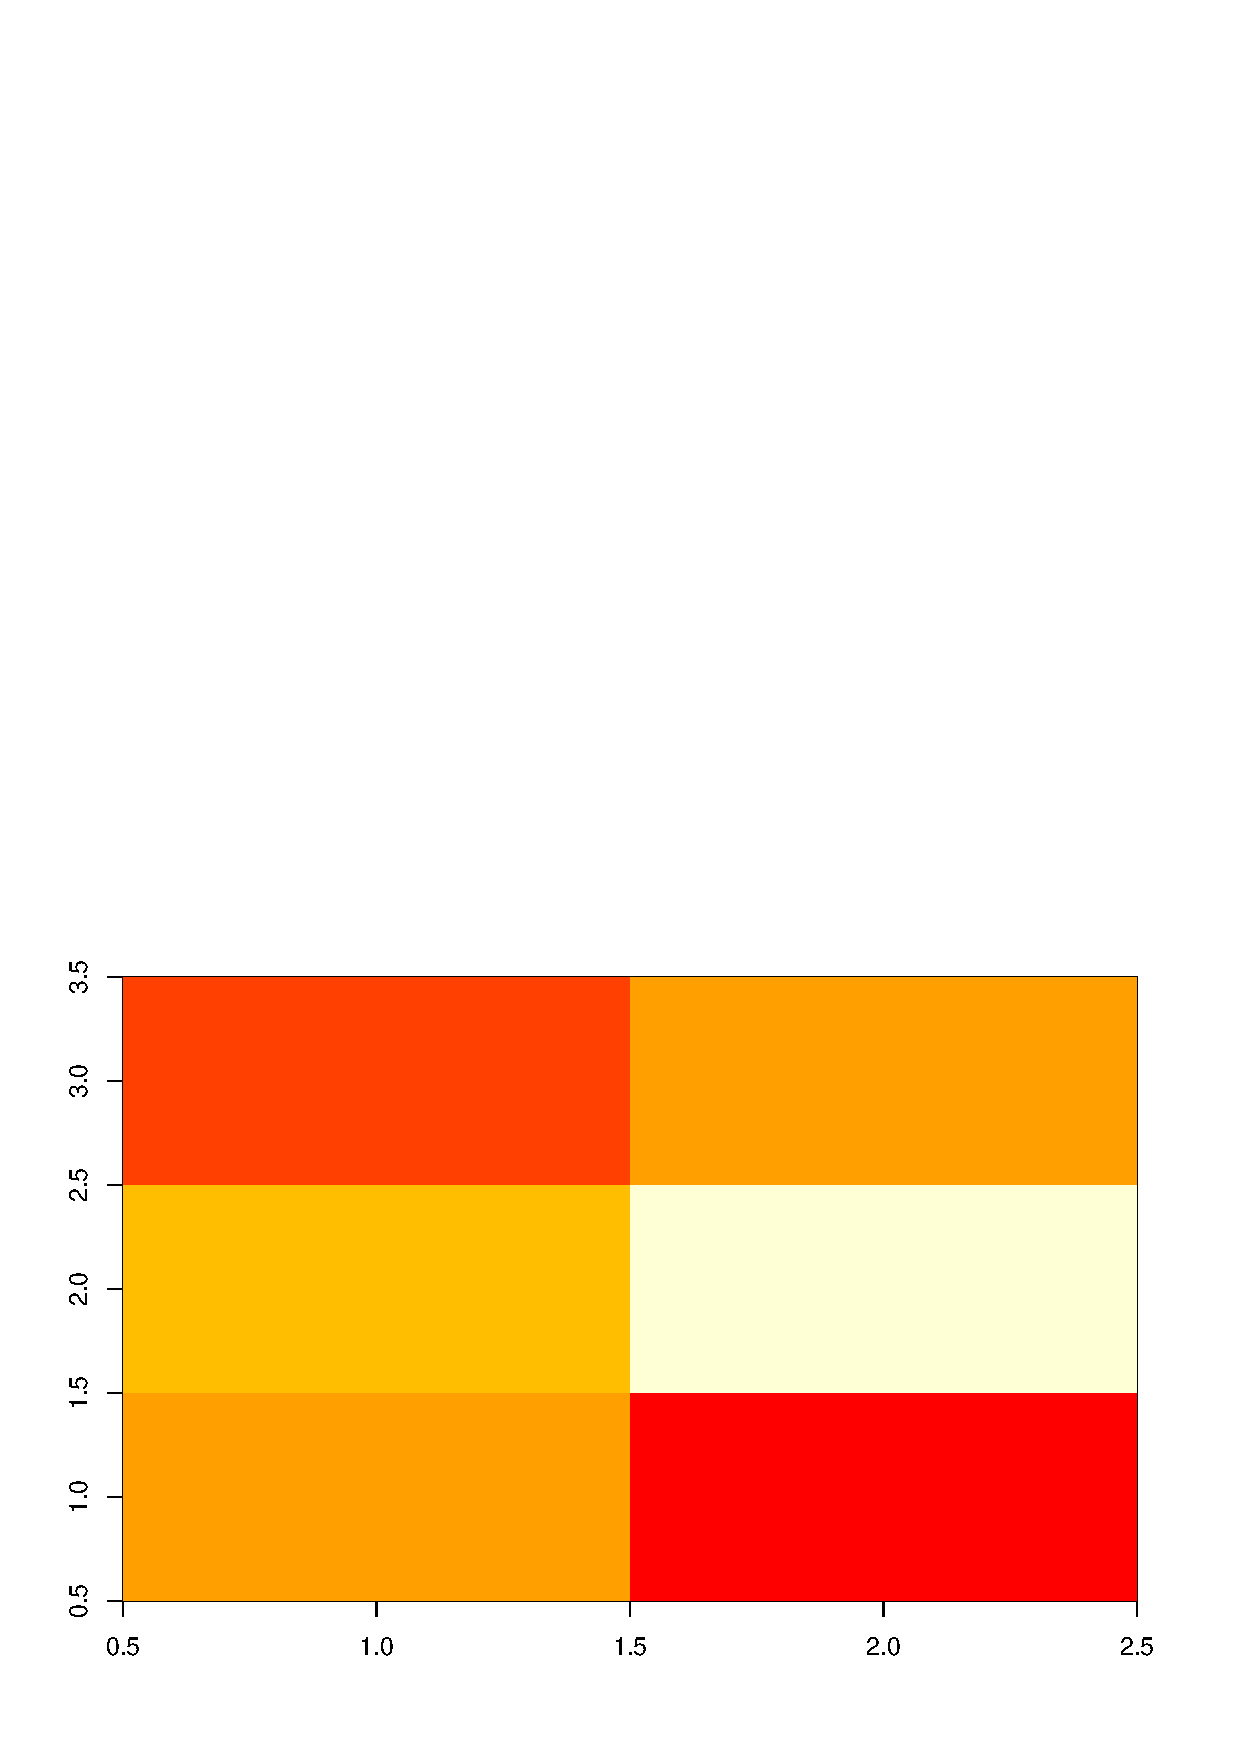
\includegraphics{image}
\caption{plot 3 of the layout is an image}
\end{figure}
\end{center}


\indent The last plot.call, given by: 
\begin{verbatim}
plot(cos, xlim = c(-pi,3*pi), n = 1001, col = 'blue', xlab='', ylab='')
\end{verbatim}
creates a cosine curve seen in figure 12.
 
\begin{center}
\begin{figure}
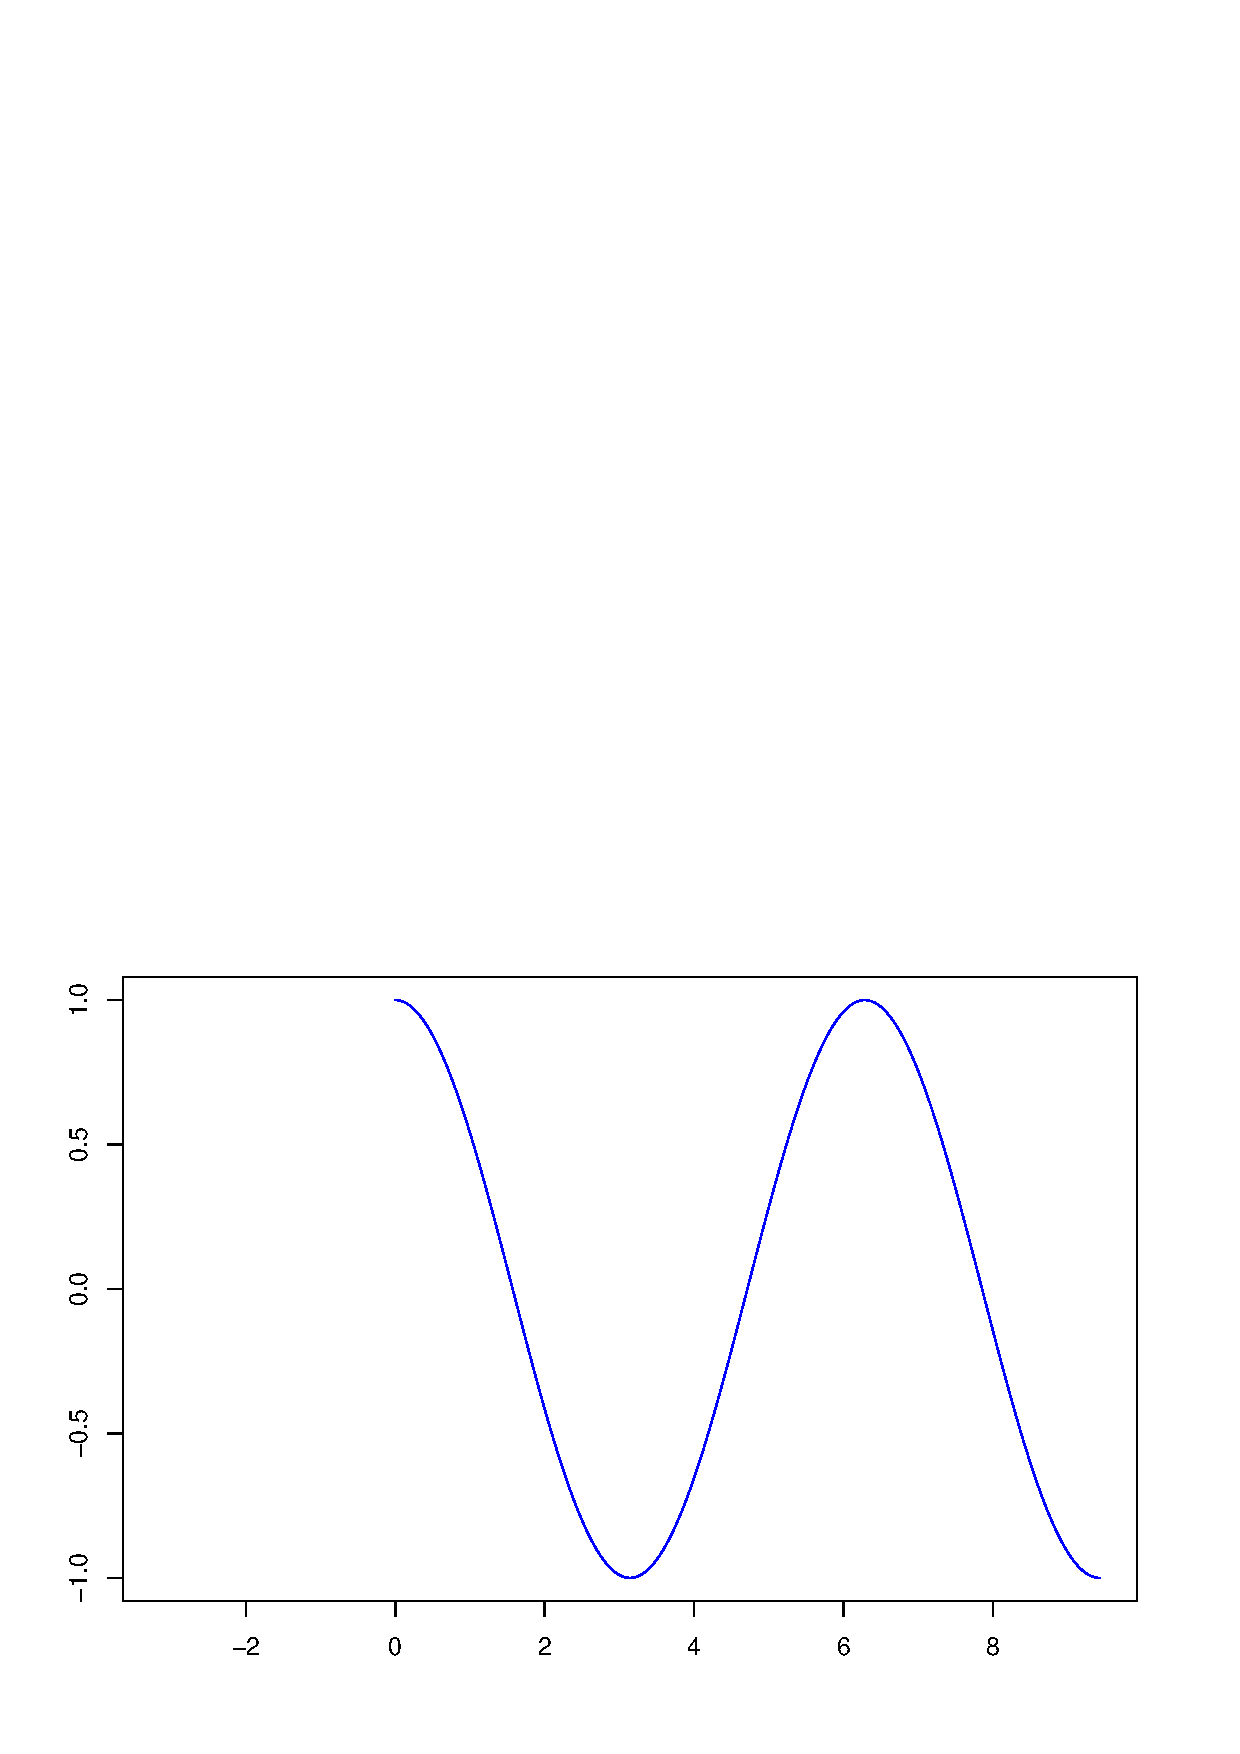
\includegraphics{sinCurve}
\caption{plot 4 of the layout is a curve}
\end{figure}
\end{center}




\indent {\bf{Note:}} Axis and additional plotting such as rectangles have not yet been plotted. Additional expressions, such as these, can be evaluated on the plots through this argument or the sendplot argument plot.extras, which will be discussed in detail later in this section. \newline

\indent Arguments of type character within any of the character strings are specified with a single quotation rather than the double quotations used originally, or vice versa (see second string's leaflab argument). Any variables used in plot calls should be in local memory before running the sendplot function. The following code initializes variables needed for above plot calls:

\begin{verbatim}
myX = c(-1,-10,1,10,-5,0)
\end{verbatim}

\indent The arguments Iflag and figType indicate features about each figure. Iflag, short for interactive flag, is a logical vector of length equal to the maximum value in mat. This tells the function which of the figures are going to have tool-tip functionality. This will get automatically updated when interactive tool-tip mappings are assigned to a figure (through makeImap). The function loops over all figures designated as interactive to make a complete image map for tool-tip functionality. figType indicates what type of graph is displayed, e.g. scatterplot, image, heatmap, tiled (feature coming soon).  This, therefore is a character vector also of length equal to the maximum value in mat. Currently, this vector is not used but is implemented in the design in preparation for a tiled heatmap setting.  \newline


\indent The initSplot arguments mai.mat and mai.prc control the margins for each plot in the display. The mai.mat argument is a numeric n x 4 matrix, where n is the length of plot calls. Each row of mai.mat is passed into the R graphics package function par specifying mai. The four columns represent the margins: bottom, left, top, and right respectively. The first row corresponds to the margins for layout designates '1', the second row to layout designates '2' and so forth. If the numeric values in the mai.mat represent a percentage of the default margins, the argument mai.prc=TRUE. The following sets up margins for Figure 7.


\begin{verbatim}
mai.mat = matrix(.5,ncol=4,nrow=4)
mai.prc = FALSE
\end{verbatim}


\indent {\bf{Note:}} If figure margins are too large, an error will occur when plotting. Error messages such a 'Error figure margins too large' can sometimes be eliminated by decreasing the values in mai.mat.


\indent plot.extras contains additional expressions or plot calls for each displayed plot. plot.extras is a list which contains sub-lists corresponding to each plot in plot.calls. Each of these sub-lists is a list of character strings to be evaluated as R functions. Additional rectangular regions are added to the first plot, a polygon is added to the second plot, and titles are added to the third and fourth plots. This is achieved with the following: 

\begin{verbatim}
plot.extras=list(
    figure1= "rect(xleft=c(3,1), ytop=c(25,5),xright=c(4,2),ybottom=c(20,0));
              title(main='A', cex=3)",

    figure2=list(c("polygon(x=c(2,2.5,3,2.5), y=c(1,2.5,1,1.5))"),
                 c( "title(main='B', cex=3)")), 
    figure3 ="title(main='C', cex=3)", 
    figure4="title(main='D', cex=3)")


\end{verbatim}



\indent Arguments of type character within any of the character strings are specified with a single quotation rather than the double quotations used originally, or vice versa (see main argument).


\indent Looking at the second plot's sub-list, there are two additional calls: one to add a title and another to make a title. 

\begin{Schunk}
\begin{Soutput}
[[1]]
[1] "polygon(x=c(2,2.5,3,2.5), y=c(1,2.5,1,1.5))"

[[2]]
[1] "title(main='B', cex=3)"
\end{Soutput}
\end{Schunk}

\indent {\bf{Note:}} Alternatively, some of the plot.extras argument could have been included in the original plot.calls argument. The original character string can contain multiple calls separated by a semicolon. The same technique can be used for the plot.extras argument. For example, the first plot.extras argument is the following:

\begin{verbatim}
"rect(xleft=c(3,1), ytop=c(25,5),xright=c(4,2),
                    ybottom=c(20,0));title(main='A', cex=3)"
\end{verbatim}

\indent Notice how there are two separate calls: one to make the rectangles and one to add a title.  If we look back at the second plot call, this technique is already used:

\begin{verbatim}
"plot(1:3,1:3, col='blue', xlab='', ylab=''); points(1:2, 2:3, col='red')"
\end{verbatim}

\indent The plot.extras arguments for the second plot (given above) could have been added to the plot.calls argument resulting in the following:

\begin{verbatim}
"plot(1:3,1:3, col='blue', xlab='', ylab=''); points(1:2, 2:3, col='red');
      polygon(x=c(2,2.5,3,2.5), y=c(1,2.5,1,1.5));title(main='B', cex=3)"
\end{verbatim}



\subsubsection{Setting the device}

This section will define the following initSplot arguments:

\begin{description}
   \item{source.plot:~}{Determines which device is used; may be NA, "ps", "png", or "jpeg"}
   \item{image.size:~}{character indicating device size value. If source.plot is "png" or "jpeg" , the argument is parsed and the dimensions are passed into the R grDevices package function png (or jpeg) as the width and height arguments. If source.plot is "ps", image.size is passed as part of a system convert command converting the postscript to the .png. The original image is resized to this dimension expanding condensed images or vice versa. }
   \item{pointsize:~}{pointsize of image. passed into device call}
   \item{res:~}{resolution of image, passed into device call if source.plot is "png" or "jpeg"}
   \item{ps.paper:~}{postscript paper argument if source.plot is "ps"}
   \item{ps.width:~}{postscript width argument (only used if ps.paper="special")}
   \item{ps.height:~}{postscript height argument (only used if ps.paper="special")}
\end{description}

\indent The source.plot argument controls what file formats are created. The interactive html file requires either a .png file or a .jpeg. If source.plot is  "png" or "jpeg" those respective files are created directly. If source.plot is "ps", a postscript file is created and then is converted into "png". If source.plot is NA or if anything else is specified, source.plot will default to "png". \newline

\indent If the source.plot argument is set to "png" or "jpeg", the width and height arguments for the device are determined by image.size. The image.size argument is a character that, in this case, is parsed on the letter "x" to retrieve the width and height in pixels. The default image.size value is a standard 800 by 1100 (See below). The initSplot argument res may also be given if the source.plot is "png" or "jpeg". This is passed into the png and jpeg functions as the res argument, representing the nominal resolution in dpi.  \newline

\indent The example uses the standard 800 x 1100 size:
\begin{verbatim}
image.size="800x1100"
\end{verbatim}

\indent If the source.plot argument is set to "ps" then a postscript file is generated and then converted (using the 'convert' command in linux or a user specified application in windows) to the PNG format. When converting, the postscript will be resized to image.size. The ps.paper, ps.width, and ps.height arguments specify the dimensions of the postscript output. If the ps.paper argument is set to a recognized format such as ``letter'' or ``a4'', then the ps.width and ps.height arguments are ignored. If the ps.paper argument is set to ``special'' then the postscript dimensions are governed by ps.height and ps.width.  \newline

\indent The initSplot argument pointsize is passed into the device function (ps, png, jpeg) as its pointsize argument. This is the default pointsize of plotting text.  

\subsubsection{Returning and Saving Splot Object}

\indent There are three arguments involved in returning or saving the Splot object. If returnVl, a logical, is TRUE the object will be returned. If saveFlag, also a logical, is TRUE, the object will be saved to a file. The file name used will be the argument saveName, by default "Splot.RData" in the current working directory. 

\subsubsection{Running initSplot}

\indent The following call will generate the Splot object for the given example:

\begin{verbatim}
Splot = initSplot(mat=mat, plot.calls=plot.calls,
                  mai.mat=mai.mat, 
                  plot.extras=plot.extras)
\end{verbatim}



\indent Now that the Splot object is created, interactive regions for tool-tip functionality may be added to the plot. 
\subsection{First Look at Data: Static plot}

\indent A brief note: it is possible to make a static version of the layout of figures created with the initSplot function call. The makeSplot function, which will be discussed in detail in section 5.4, may be run at any time on the Splot object. If makeImap has not been utilized yet, or if makeSplot is run with the argument makeInteractive as FALSE,  then a static layout of plots is generated.

\begin{verbatim}
Splot = makeSplot(Splot, fname.root="FirstLookEx", 
                  makeInteractive=FALSE, returnObj=TRUE)

\end{verbatim}


\indent This may be handy to verify the figure is generated to preference before adding interactive data, or to test if the interactive data is added to the plot correctly. If the user is using R plotting functions that generate some output object, the output will also be saved to the Splot object. This may be useful for finding information or indices for tool-tip regions.  

\subsection{makeImap: Adding Interactive Tool-tip Regions}

\indent The Splot object has been created. Now lets add to tool-tip functionality. The makeImap function may be run any number of times. This function adds data that will be included in the tool-tip display of the HTML. The following is an example function call:

\begin{verbatim}
makeImap(Splot, x.pos, y.pos,
         figure=1,
         xy.type=NA, 
         x.right.pos=NA, y.bottom.pos=NA, 
         spot.radius = 5, 
         x.labels=NA,y.labels=NA,xy.labels=NA,
         x.links=NA, y.links=NA,xy.links=NA,
         asLinks=NA,
         font.type="Helvetica",font.color="black", 
         font.size="12",bg.color='#D6E3F6',  
         fname.root="Splot",dir="./",
         automap=TRUE,automap.method="mode",
         bb.clr=NA,bb.cex=2,               
         returnVl=T,saveFlag=F,saveName="Splot.RData")
\end{verbatim}

\subsubsection{specifying the interactive points}

This section will define the following makeImap arguments:
\begin{description}
   \item{figure:~}{numeric value of which figure to add interactive data}
   \item{xy.type:~}{the region type. Acceptable types are points, image.midpoints, image.boundaries, image.box, circle, rect, or polygon}
   \item{x.pos:~}{x axis position of interactive region; the left x axis position if xy.type is rect}
   \item{y.pos:~}{y axis position of interactive region; the top y axis position if xy.type is rect}
   \item{x.right.pos:~}{If xy.type is rect, the right x axis position. If other xy.type, this argument is not utilized}
   \item{y.bottom.pos:~}{If xy.type is rect, the bottom y axis position. If other xy.type, this argument is not utilized}
   \item{spot.radius:~}{The radius of the interactive points in pixels. This is utilized when xy.type is circle or points.}
\end{description}


\indent The makeImap function works on one figure at a time. It is necessary then to specify the figure (using the 'figure' argument) for a particular run. This should be a numeric value in the range of 1:maximum number of figures in the layout.  The number will correspond to the region in mat; see section 5.1 or figure 8. \newline

\indent The user must specify the region[s] type and location[s] of the interactive tool-tip functionality. The makeImap function xy.type is the argument for the region type. Currently supported xy.types are points, image.midpoints, image.boundaries, image.box, circle, rect, and polygon. Points, image.midpoints, image.boundaries and circles result in an HTML circle image area. image.box and rect result in an HTML rect area. Polygon results in a HTML poly area. The xy.type argument is important in determining correct mappings between the region location[s] in the R plots and pixel mappings. For HTML circle regions created through xy.type circle or points, the x and y coordinates of the center[s] of the circle[s] should be given in the makeImap arguments x.pos and y.pos, as well as the spot radius to use in the argument spot.radius. The xy.types image.midpoints and image.boundaries are special as it is assumed that the points are referring to regions within an R image (heatmap) plot. The value image.midpoints assumes that the x.pos and y.pos coordinate locations correspond to the middle of the grid lines of an image. The value image.boundaries assumes the x.pos and y.pos coordinate locations are the designated grid lines of an image. When image.boundaries is used, the function will calculate the midpoints to use for interactive locations. To clarify, the x.pos and y.pos contain matching x,y point coordinates. The first circle is (x[1], (y[1]), the second (x[2], y[2]), and so forth. The spot.radius argument is utilized for image.midpoints and image.boundaries as well as circle and points. The spot.radius may be a single value that will be used for all points, or it may be a numeric vector of length equal to the total number of interactive circle regions. \newline

\indent There are two xy.type options to create rectangular HTML regions: image.box and rect. When xy.type is rect, x.pos and y.pos have a slightly different meaning. The x.pos and y.pos are not simply the x and y coordinates; they are the left most x coordinate and top y coordinate for the rectangular region[s]. Two additional makeImap arguments are used, x.right.pos and y.bottom.pos, to give the right most x coordinate and bottom y coordinate of the rectangular region[s]. For example, the first box would have the following vertices: (x.pos[1], y.bottom.pos[1])(x.pos[1], y.pos[1])(x.right.pos[1], y.pos[1])(x.right.pos[1], y.bottom.pos[1]). The type image.box, as the name suggests, assumes the coordinates are referring to an image. Only the x.pos and y.pos arguments are used, not x.right.pos or y.bottom.pos, and it is assumed they are the locations of grid lines of an image (just like image.boundaries).\newline

\indent Adding a polygon region is also a little different. Only one polygon figure may be added at a time. The x.pos and y.pos therefore hold the x and y coordinates of all vertices in the polygon. If the polygon does not close, i.e. the first and last vertices are the same, the starting coordinates will be added. \newline

\indent It is important to note that the interactive regions are independently determined from the plots displayed. It is therefore possible to make an entire data set interactive, any subset of data interactive, or to have hidden interactive regions. 

\subsubsection{specifying tool-tip data}

\indent Now that the interactive regions have been identified, data can be attached to regions to display in tool-tip. The following makeImap arguments hold data and links:
\begin{description}
   \item{x.labels:~}{data frame of n x m which contains values relating to the x.pos.}
   \item{y.labels:~}{data frame of n x m which contains values relating to the y.pos.}
   \item{xy.labels:~}{list of matrices. All matrices should be of n x m. point (x.pos and y.pos) specific}
   \item{x.links:~}{data frame of n x m which contains web addresses for links relating to the x.pos}
   \item{y.links:~}{data frame of n x m which contains web addresses for links relating to the y.pos}
   \item{xy.links:~}{list of matrices. All matrices should be of n x m which contain complete web address for point (x.pos and y.pos) specific links}
   \item{asLinks:~}{character vector which contains complete web address for points that should be treated as hyperlinks}
\end{description}

\indent In general, as the names suggest, x.labels, y.labels and xy.labels hold data and the corresponding link arguments hold web address links. The dimensions of the matrices depend on the xy.type: points, circle, image.midpoints, image.boundaries, image.box, rect, and poly. x.labels and x.links hold data specific to the x set of points or x.axis, just as y.labels and y.links is y specific data. The xy.labels and xy.links arguments hold data xy specific. Let's begin by looking at the lengths and dimensions of these arguments when xy.type is circle,points, or rect. It this case, since x.pos and y.pos refer to the same point location, x.labels, y.labels, and xy.labels (and x-,y-,xy- links) are essentially the same. These matrices should be of length n by m where n is equal to the length of x.pos (or y.pos) and $m$ is the number of columns represent data to be included in the tool-tip.\newline

\indent  The distinction between the x.labels, y.labels, and xy.labels arguments (and respective links) can be seen when the xy.type is image.midpoints, image.boundaries, or image.box. Images may have an unequal number of x.pos and y.pos values. x.labels and x.links refer to data specific to the image x-axis, or the locations in x.pos. There are some slight differences when using image.midpoints over image.boundaries or image.box. When xy.type is image.midpoints, x.labels and x.links are n by m matrices where n is equal to the length of x.pos and the columns represent data to be included in the tool-tip. Similarly, y.labels and y.links refer to data specific to the image y-axis and are n by m matrices where n is equal to the length of y.pos. The xy.labels and xy.links arguments contain data that is specific to both x.pos and y.pos. These arguments are lists of matrices n by m where n is equal to the length of y.pos and m is equal to the length of x.pos. When image.boundaries or image.box is used as xy.type, instead of the length of x.pos or y.pos, they become the length of x.pos minus one and the length of y.pos minus one. \newline

\indent The last xy.type is poly. Adding polygons are different from the other types in that only one may be added at a time. All data.frames or matrices are therefore 1 by n: one object with n desired descriptive data. \newline

\indent  The argument asLinks contains web addresses that will be linked to the interactive region directly (i.e. when you left click hovered over the region it will redirect you to this site) or NAs that represent no hyperlink for a region.  When xy.type is circle, point, or rect the length of asLinks may be the length of x.pos (or y.pos)  or 1.  If the length of asLinks is 1, that value will be repeated for every region of the dataset. The order in asLinks should be the same as the order of x.pos (or y.pos).  When xy.type is referring to an image, there are a few other options for asLinks.  The argument may be of length equal to the x.pos (x specifics links) which will be repeated for every point with the corresponding x.pos; similarly it may be of length y.pos for y.specific links that will be repeated. asLinks may also be of length one.  A matrix or data.frame that would correspond to the image regions may also be used as asLinks. A vector of length equal to the length of x.pos by the length of y.pos may also be used.  In this case the order should correspond to the order that would occur if the matrix was converted into a vector. {\bf{Note:}} If the x.pos and y.pos are boundaries of grid-lines instead of the midpoints, the above description should be the length of x.pos minus one and the length of y.pos minus one instead of the lengths of x.pos and y.pos. Again, when xy.type is a poly, asLinks will also be a single entry of either a complete web address or NA. 

\subsubsection{altering tool-tip display}
\indent The following features can be changed in the tool-tip display window:  font style, font color, font size, and background color. The function arguments that handle these features are:
 
\begin{description}
\item{font.type:~}{character indicating the name of the font to use. There are currently three supported font types: Arial, Helvetica and sans-serif}
\item{font.color:~}{character giving the name or in the format of '\#------' of the desired font color}
\item{font.size:~}{numeric indicating the size of the font }
\item{bg.color:~}{character indicating the name or in the format of '\#------' of the desired background color}
\end{description}

These options are given so the user has more control over how information is displayed. The tool-tip window size will automatically readjust to fit the data desired with the given size.

\subsubsection{Generated objects and Files}

The following arguments are involved in creating and saving objects and files:
\begin{description}
\item{fname.root:~}{character, base name to use for file[s] created}
\item{dir:~}{character, directory path for where the file[s] should be created}
\item{returnVl:~}{logical, indicates if the Splot object should be returned with updated information}
\item{saveFlag:~}{logical, indicates if the Splot object should be saved as a file}
\item{saveName:~}{character, full name (including directory path if desired), to save Splot object if saveFlag is TRUE}
\end{description}

\indent In the automatic mapping portion of this function, .png and .tif files are created. The fname.root argument gives the base name for all these files to ensure that previously generated files are not accidentally overwritten. The dir argument is added as a prefix to the fname.root to create a full path name for the files generated. Certain values are added to the Splot object as well as the data for the tool-tip display. If the user wishes to return the Splot object returnVl should be set to TRUE. If the user wishes to save the Splot object to a file to load again later, saveFlag should be set to TRUE. The file will be given the name saveName. This argument should be the complete path name (i.e. the directory structure should be included otherwise it is saved in the current working directory). 

\subsubsection{Comments on automap feature and  helpful hints}

\indent Currently the new version of sendplot only has an automap feature. Ways to override the automap will be coming as extensions in future versions. The argument automap therefore must be TRUE at all times. The automap method utilizes the R library rtiff and pixmap. An image is created and then another image is created with the addition of two points at the graph boundary locations. These images are converted to tif files using linux built in convert options {\bf{Note:}} This means the current version also only works on linux. Windows compatible extensions will be released in future versions of the package. The images are compared and the regions that are different, hence the bounding locations of the plot, are found. The locations are determined through either a median or mode method. This can be set through the argument automap.method. The median will take the middle of all the rows and columns that are different as the central location of the desired bounding points. The mode method looks for the most common areas and takes the middle of that region. \newline

\indent There are a few reasons why the automap method may throw errors. These helpful hints should aid in clarification and resolutions. A common cause of error is that the graphing region is two small based on margin size and the location allocation given in the mat for layout. If the plotting region is too small, the points that are added will be less than a pixel and will not appear as a region of difference when images are compared. Likewise, if the plotting region is too large, and the point size is small, the point will also be less than a pixel and not be recognized.  Margins and matrix allocations may be altered. The user may also try increasing or decreasing the size of the points added for automatic detection. This is controlled through the argument bb.cex. This should be the numeric point size of the bounding points. Another common cause for error is the color of the plot at the plot boundary may be the same color as the added points. This will also cause no change to be recognized and an error to occur. The color of the bounding points may be changed through the bb.clr argument. This should be a character value with the name of the color. By default the application tries blue, red, black, white, and green. It will stop if any one of the colors works properly. 

\subsubsection{Examples of makeImap}

This section will use the makeImap function to add various sets of data to the example seen in figure 7. 
\vspace{5mm}

\indent {\bf{CREATING LAYOUT FIGURE 1}} 


\vspace{5mm}

\normalsize

This example will add three interactive data sets to figure 1: two sets of points/circle and set of rectangles. 

In section 5.2, a static version of a layout of plots is generated. This allows the Splot object to save output from the R boxplot function call. This output can be used to add data to the plot. For example, perhaps the median values of each group: 


\begin{verbatim}
 xvec = 1:6
 yvec = Splot$plot.output[[1]]$stats[3,]
\end{verbatim}

The xvec and yvec will be the locations of our interactive regions, and therefore be passed into makeImap as x.pos and y.pos respectively. Now data will be added to each group using the x.labels, x.links, and asLinks arguments. 

Three pieces of data will be added through the x.labels argument: an identifier for the group (i.e. boxplot.group1, boxplot.group2, ...), the median value (i.e. yvec), and, since we will be using asLinks to make certain points interactive, a label to indicate as such. x.lbls is a data.frame of the dimension n by m, where n is the number of points, in this case 6, and m columns of information, in this case 3. The names, or column names, of the data frame will be used as the label in the tool-tip display.   


\begin{verbatim}
x.lbls = as.data.frame(matrix(c("boxplot.group1","boxplot.group2",
                                "boxplot.group3","boxplot.group4",
                                "boxplot.group5","boxplot.group6", 
                                as.character(yvec),
                                "not a link", "not a link", 
                                "im a link", "im a link",
                                "not a link", "not a link"),
                        ncol=3))
names(x.lbls) = c("x.Label.1","x.Label.2", "asLinks")  
\end{verbatim}

Similar to the x.labels argument is the x.links argument. This will add hyperlinks to the tool-tip display. Data in this data.frame should be complete address of the link (i.e http://www.buffalo.edu) or NA if there should not be a link. In this example, the first three groups will have a link.1 that links to the University at Buffalo homepage and all of the groups will have a link.2 with two hyperlinks: one to the University at Buffalo homepage and one to the Center for Excellence in Bioinformatics and Life Sciences homepage. Notice how the two links for link.2 are given: it is a single character string but the two links are separated with a comma. 


\begin{verbatim}
x.links = as.data.frame(matrix(rep(NA, 12), nrow=6))
x.links[1:3,1] = "http://www.buffalo.edu"
x.links[,2] = "http://www.buffalo.edu, http://www.bioinformatics.buffalo.edu/"
names(x.links) = c("link.1", "link.2")
\end{verbatim}

The asLinks argument makes the regions themselves hyperlinks. For this example, the third and forth groups will be hyperlinks to the University at Buffalo Biostatistic Department software web-page. 


\begin{verbatim}
asLinks = c(NA, NA, "http://sphhp.buffalo.edu/biostat/research/software/index.php", 
           "http://sphhp.buffalo.edu/biostat/research/software/index.php", NA, NA)
\end{verbatim}

Now that x.lbls, x.links, and asLinks have been defined, they may be passed into the makeImap function to make the boxplot groups interactive. 



\begin{verbatim}
Splot = makeImap(Splot, figure=1, xy.type="points",
                 x.pos=xvec, y.pos=yvec,
                 x.labels = x.lbls, asLinks = asLinks, x.links=x.links, 
                 fname.root="sendPlotEx", spot.radius=25)
\end{verbatim}

The boxplot graph corresponds to figure 1 as defined by the layout in figure 8. In this case the region is going to be a point or circle; point is used. The spot radius can be adjusted to allow for a larger interactive region on the HTML page. It is possible to change the tool-tip display font, font size, font color or background color. In the above example, defaults are used. Figure 13 shows the second points tool-tip display.

 
\begin{center}
\begin{figure}

\includegraphics[width=1.5in, height=1in]{tip1}
\caption{boxplot, group2, tool-tip display for layout figure 1.}
\end{figure}
\end{center}


In the boxplot graph, figure 9, notice how there are two outlier points. Now we will add data to the first outlier point. Only one point is going to be given, therefore all data.frames are of the dimension 1 by n. The interactive region will still be added to figure 1 and the xy.type appropriate will either be a point or circle; point was used in the last example, so we will use circle. The x.pos and y.pos values will again be taken from the plot output generated from running the boxplot function. For points and circles, the x and y values are equivalent, therefore x.labels and y.labels are interchangeable; we include both an x.labels and y.labels argument although they may have been combined into one 1 by n data.frame. The x.labels argument is including data for the type of region and that the point is a link which will be set through asLinks. The y.labels argument is giving information about the value of the outlier point and details about the tool-tip display. In this example we will be changing all of the default tool-tip settings. Notice the makeImap arguments appropriately named for font.type, font.size, font.color, and background color; these are the arguments that change the tool-tip features. In this example we change the font type, increase the font size, change the font color to hotpink, and change the background color to blue.    



\begin{verbatim}
Splot=makeImap(Splot, figure=1, xy.type="circle", 
               x.pos=Splot$plot.output[[1]]$group[1], 
               y.pos=Splot$plot.output[[1]]$out[1],
               x.labels = list(Xlabel1.xyType="point", Xlabel2.asLinks="im a link"),
               y.labels = list(ylabel1.yValue="7", tooltip.font="arial",
                               tooltip.size="20",tooltip.fontcolor="hotpink",
                               tooltip.background="blue"),
               asLinks = "code.html/interactiveFigure1.html", 
               fname.root="sendPlotEx", spot.radius=20,
               font.type="arial", font.size="20", font.color="hotpink", bg.color="blue")
\end{verbatim}

The tool-tip designed is shown in figure 14. 

 
\begin{center}
\begin{figure}

\includegraphics[width=2.2in, height=1.7in]{tip2}
\caption{boxplot, outlier tool-tip display for layout figure 1.}
\end{figure}
\end{center}


The final interactive regions that will be added to the first figure (figure=1) will be for the extra rectangular regions plotted through the initSplot plot.extras argument. To recall the plot.extras call was: 

\begin{verbatim}

>Splot$plot.extras[1]

$figure1
[1] "rect(xleft=c(3,1), ytop=c(25,5),xright=c(4,2), ybottom=c(20,0));
title(main='A', cex=3)"

\end{verbatim}

Notice, the bounding locations of both rectangles are already known since they were user specified. The x.pos and y.pos arguments become the rect function arguments x.left and y.top respectively. The makeImap function has two additional arguments for the case when a rectangular region is used: x.right.pos and y.bottom.pos. The rect function arguments xright and ybottom are used for these values respectively. The xy.type is now going to be rect instead of the previously used circle or point. Again data is added through the x.labels, y.labels, x.links, asLinks, etc. arguments. All data.frames will be of dimension 2 by n since there are two rectangular regions. The x.labels argument will give a label, and coordinates for the rectangular regions as well as an indication if asLinks was used. The argument y.labels will give information on the changes of tool-tip settings. In this case the font color is specified as cyan, and the background color is specified as black. Notice although there are two regions being specified the asLinks argument is a single value. This value will be repeated for all regions: in this case twice. The x.links data.frame will also be utilized. As the x.links data.frame is set up the first rectangle will have two links: the UB link and the buildings links. The second rectangle will also have two links but it will only have the buildings links and the stats link. 


\begin{verbatim}
x.links = as.data.frame(matrix(rep(NA, 6), nrow=2))
x.links[1,1] = "http://www.buffalo.edu"
x.links[,2] = "http://www.buffalo.edu, http://www.bioinformatics.buffalo.edu/"
x.links[2,3] = "http://sphhp.buffalo.edu/biostat/"
names(x.links) = c("UB", "buildings", "stats")


Splot = makeImap(Splot, figure=1, xy.type="rect", 
                 x.pos=c(3,1), y.pos=c(25,5),
                 x.right.pos=c(4,2),  y.bottom.pos=c(20,0),  
                 x.labels = as.data.frame(list(Xlabel.1=c("rect.1","rect.2"),
                      Xlabel.2.coordinates=c("3,20-3,25-4,25-4,20","1,0-1,5-2,5-2,0"),
                      asLinks=c("im a link", "im a link"))),
                 y.labels = list(tooltip.size=c("15","15"),
                                 tooltip.fontcolor=c("cyan","cyan"), 
                                 tooltip.background=c("black","black")),
                 asLinks = "http://sphhp.buffalo.edu/biostat/",
                 fname.root="sendPlotEx",
                 x.links=x.links, font.size=15, font.color="cyan", bg.color="black")
\end{verbatim}

Figure 15 show the tool-tip display for one of the rectangles.

 
\begin{center}
\begin{figure}
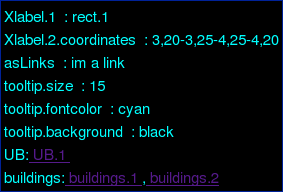
\includegraphics[width=2.2in, height=1.7in]{tip3}
\caption{boxplot, rectangle tool-tip display for layout figure 1}
\end{figure}
\end{center}


\vspace{5mm}

\indent {\bf{CREATING LAYOUT FIGURE 2}} 


\vspace{5mm}

\normalsize

This example will add three interactive data sets to figure 2: two sets of points and a polygon. 

The points in these plots are added directly through the plot.calls. Looking at the original plot.calls setting for figure 2:

\begin{verbatim}

>Splot$plot.calls[2]

[1] "plot(1:3,1:3, col='blue', xlab='', ylab=''); points(1:2, 2:3, col='red')"

\end{verbatim}


First, interactive data will be added for the set of three blue points. The x.labels argument will add a label for the xy.type (i.e point1, point2, point3) and an indication if the point is a link, which is determined by the asLink argument. The y.labels argument is also used to relay information about the tool-tip display changes; the font is now larger and green, and the background is transparent. Notice to get a transparent background the bg.color is set to an empty string.  The y.link argument will add hyperlinks to the tool-tip. In this example the first point will have two hyperlinks: the UB link and the department link. The second point will have all three: UB, buildings, and department links. The third point will only have two links: the building and department links. Note: The data set is a set of points and therefore x.labels and y.labels may be used interchangeably, as well as x.links and y.links. x.labels and y.labels therefore could be combined into one larger data.frame. The asLinks argument determines if the points themselves should be hyperlinks. If NA the point is not a hyperlink, otherwise values should be complete web addresses. In this case, each point is a link to a different site either the University at Buffalo, Center for Excellence in Bioinformatics and Life Sciences, or the University at Buffalo Biostatistics web-pages.


\begin{verbatim}
x.lbls = as.data.frame(list(xLabel1.xyType=c("point1", "point2", "point3"),
                            xLabel2.asLinks=c("im a link", "im a link", "im a link")))
y.links = as.data.frame(matrix(rep(NA, 9), nrow=3))
y.links[1:2,1] = "http://www.buffalo.edu"
y.links[2:3,2] = "http://www.buffalo.edu, http://www.bioinformatics.buffalo.edu/"
y.links[,3] = "http://sphhp.buffalo.edu/biostat/"
names(y.links) = c("UB", "building", "department")
asLinks=c("http://www.buffalo.edu",
          "http://www.bioinformatics.buffalo.edu/",
          "http://sphhp.buffalo.edu/biostat/")

Splot = makeImap(Splot, figure=2, xy.type="circle",
                 x.pos=1:3, y.pos=1:3,
                 y.labels = list(tooltip.fontcolor=c("green", "green", "green"),
                     tooltip.size=c("14", "14", "14"),
                     tooltip.background=c("transparent", "transparent", "transparent")), 
                 asLinks = asLinks, x.labels = x.lbls,
                 fname.root="sendPlotEx", y.links=y.links,
                 bb.cex=5, spot.radius=20,
                 font.color="green",bg.color="", font.size="14" )

\end{verbatim}

Figure 16 shows the tool-tip for the first point of the dataset. The entire plot is displayed to better see the transparent effect of the tool-tip background. 

\begin{center}
\begin{figure}
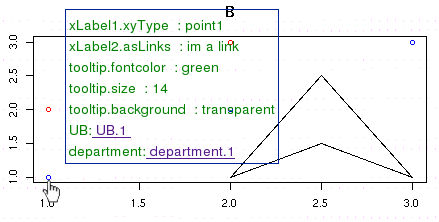
\includegraphics[width=3.3in, height=2in]{tip4}
\caption{scatterplot, point tool-tip display showing transparency for layout figure 2.}
\end{figure}
\end{center}



Now interactive data will be added to the other two red points. Similar data to the above will be added, however the tool-tip display will use default settings, there will not be any hyperlinks included, and none of the points will act as hyperlinks. 


\begin{verbatim}
y.lbls = as.data.frame(list(xLabel1.xyType=c("point1", "point2"), 
                            xLabel2.asLinks=c("im not a link", "im not a link")))
Splot = makeImap(Splot, figure=2, xy.type="circle", 
                 x.pos=1:2, y.pos=2:3,
                 x.labels = list(tooltip=c("default settings", "default settings")),
                 y.labels = y.lbls,
                 fname.root="sendPlotEx", bb.cex=5,spot.radius=15)
\end{verbatim}

The tool-tip displayed in figure 17 is what is generated. 

\begin{center}
\begin{figure}
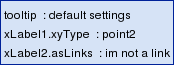
\includegraphics[width=1.6in, height=.6in]{tip5}
\caption{scatterplot, point tool-tip display dataset 2 for layout figure 2.}
\end{figure}
\end{center}




A new unique region, a polygon,  is included in figure 2. The xy.type therefore becomes polygon. It was added through the plot.extras argument and therefore the vertice locations are known. These locations become the x.pos and y.pos arguments. Recall:

\begin{verbatim}

>Splot$plot.extras[3]

$figure2
[1] "polygon(x=c(2,2.5,3,2.5), y=c(1,2.5,1,1.5));title(main='B', cex=3)"

\end{verbatim}

Notice given the above vertices, the polygon would be open. This application will assume all polygons are closed figures and add in the segment to close automatically (i.e x=c(2,2.5,3,2.5,2) and y=c(1,2.5,1,1.5,1). \newline
\indent Only one polygon region may be added at a time. All data.frames are going to be of the dimension 1 by n, where n is desired display information. The tool-tip will have increased san-serif purple font larger than the default setting. The polygon will also contain links to three websites and will link itself to the University at Buffalo Biostatistics web-page.  


\begin{verbatim}
x.links = as.data.frame(matrix(rep(NA, 3), nrow=1))
x.links[,1] = "http://www.buffalo.edu"
x.links[,2] = "http://www.bioinformatics.buffalo.edu/"
x.links[,3] = "http://sphhp.buffalo.edu/biostat/"
names(x.links) = c("UB", "CoE", "biostats")



Splot = makeImap(Splot, figure=2, xy.type="polygon",
                 x.pos=c(2,2.5,3,2.5), y.pos=c(1,2.5,1,1.5),
                 x.labels = as.data.frame(list(xLabel.xyType = "Polygon")), 
                 asLinks="http://sphhp.buffalo.edu/biostat/",
                 x.links=x.links,fname.root="sendPlotEx", bb.cex=5,
                 y.labels = as.data.frame(list(yLabel1.asLinks="Im a link",
                                          tooltip.fonttype="san-serif",
                                          tooltip.fontsize="30",
                                          tooltip.fontcolor="purple" )), 
                 font.size=30, font.type="sans-serif", font.color="purple")
\end{verbatim}

Figure 18 shows the tool-tip for the polygon region

\begin{center}
\begin{figure}
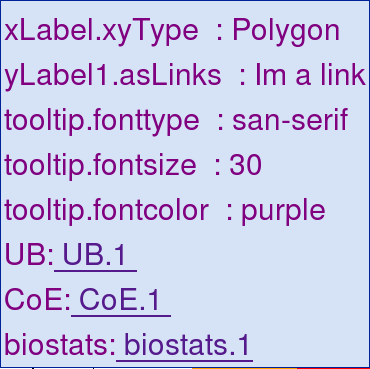
\includegraphics[width=2in, height=2.3in]{tip6}
\caption{scatterplot, polygon tool-tip for layout figure 2}
\end{figure}
\end{center}



\vspace{5mm}

\large \indent {\bf{CREATE LAYOUT FIGURE 3}} 

\vspace{5mm}

\normalsize

There are a few different options to make the image plot interactive. The options will determine whether the bounding locations or the central location for the measurements are known.  

To recall, the plot.calls argument for figure 3:

\begin{verbatim}

>Splot$plot.calls[3]

[1] "image(1:2,1:3, z=matrix(myX,ncol=3,nrow=2), xlab='', ylab='')"

\end{verbatim}

The values for x and y represent where the values at z were taken; they therefore are the central locations for the measurements. If these values are used for x.pos and y.pos the xy.type should be image.midpoints. The midpoint of each rectangular region will be interactive for a certain specified spot.radius. Figure 19 shows an example of the interactive region within an image when using image.midpoint. 

\begin{center}
\begin{figure}
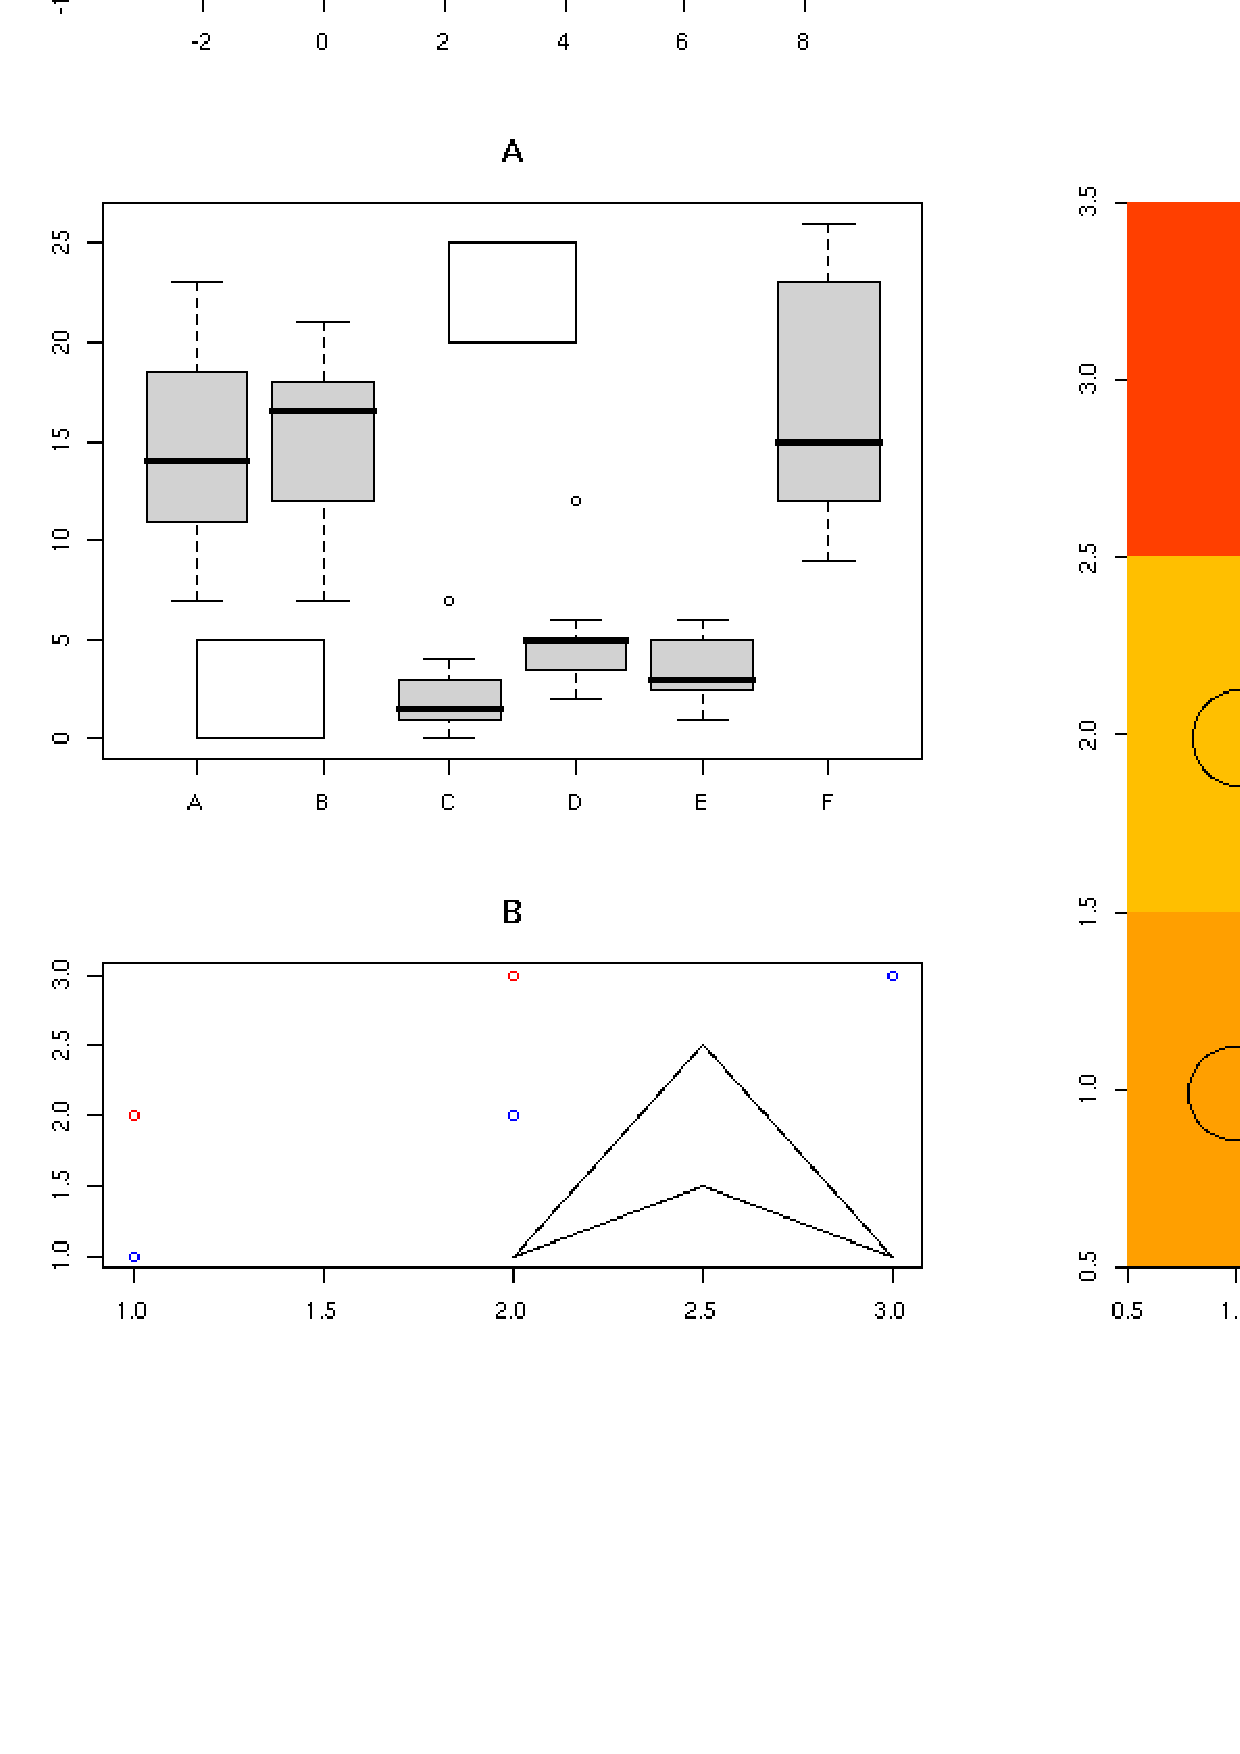
\includegraphics[width=3in, height=4in]{imageMidEx}
\caption{Example showing the interactive region within an image when image.midpoints is used. Note: black circles only indicate region that is interactive they do not actually appear in the image.}
\end{figure}
\end{center}

The other xy.type options for an image are image.boundaries and image.box. These options are used when the boundary locations are known for an image. In figure 19, the bounding grid locations for x are 0.5, 1.5, and 2.5 while the bounding grid locations for y are 0.5, 1.5, 2.5, and 3.5. These are the x.pos and y.pos values if xy.type is image.boundaries or image.box.  The value image.boundaries would result in an interactive region seen in figure 19. The function uses the boundary locations to compute the midpoint region. When image.box is used, the boundary locations are used to generate rectangular interactive regions. Figure 20 shows the example interactive region for an image when this option is utilized.     

\begin{center}
\begin{figure}
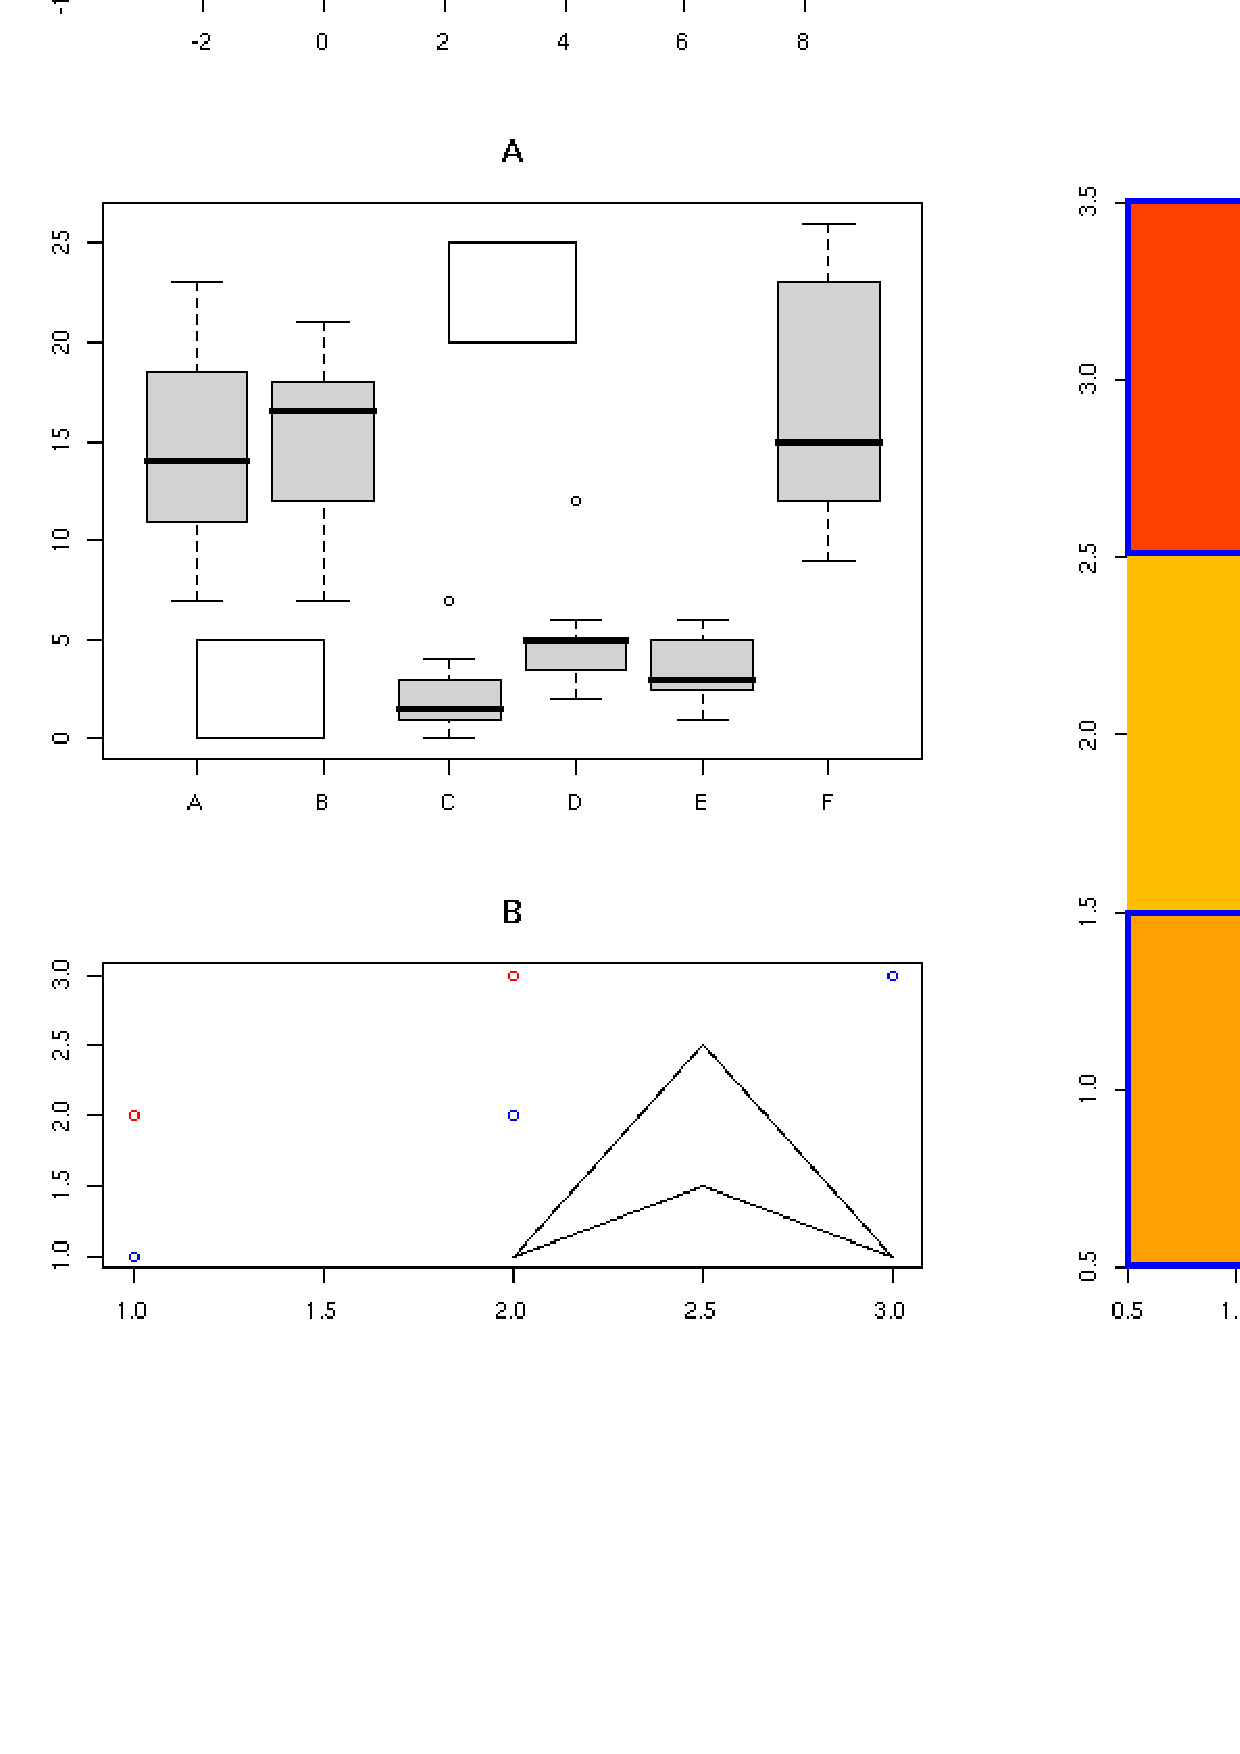
\includegraphics[width=3in, height=4in]{imageBoxEx}
\caption{Example showing the interactive region within an image when image.box is used. Note: blue rectangles only indicate a region that is interactive they do not actually appear in the image.}
\end{figure}
\end{center}

Interactive data will now be added to the image using the x.labels, y.labels, and xy.labels arguments. The difference between the x.labels, y.labels, and xy.labels arguments may really be distinguished when adding data to an image plot where the x and y values are not of equal length and are not representing the same point. The x.labels argument hold data specific to the x axis points. In this case there are two x values so x.labels is of the dimension 2 by n. Two pieces of x.specific data will be added: an indication that the xy.type is image.box, and an indication of which X value the image is referring. 



\begin{verbatim}
x.lbls=as.data.frame(list(xLabels.xy.type= c("image.box", "image.box"),
                          xLabels.1 = c("X.1", "X.2")))
\end{verbatim}

The y.labels argument behaves exactly as the x.labels argument, only with respect to the y values or y.axis. In this case the y.labels argument will be of the dimension 3 by n. Only one y specific data will be added: an indication of which Y value the image is referring. 


\begin{verbatim}
y.lbls=as.data.frame(list(y.Labels = c("Y.1", "Y.2", "Y.3")))
\end{verbatim}

The xy.labels argument contains data specific to both x and y data points of an image. All matrices within the xy.labels argument should be the same dimension as the matrix of values passed in the image call for z: in this example 3 by 2. 

 

\begin{verbatim}
xy.lbls=list(XY.label = matrix(c("image.box1","image.box2", "image.box3",
                                 "image.box4","image.box5","image.box6"),ncol=2), 
             XY.label2 = matrix(c("X1.Y1","X1.Y2", "X1.Y3",
                                  "X2.Y1","X2.Y2","X2.Y3"),ncol=2))
\end{verbatim}

Hyperlinks may be added to the tool-tip display through the x.links, y.links, and xy.links arguments.These arguments behave exactly the same as x.labels, y.labels, and xy.labels respectively;  the only difference is the data given in the links arguments should be complete web addresses. The following will have an x specific link for the first x value only and y specific links for the second and third y value. 



\begin{verbatim}
x.links=as.data.frame(list(X.links.1 = c("http://www.buffalo.edu", 
                                         NA)))
y.links=as.data.frame(list(Y.links.1 = c(
                 NA,
                "http://www.buffalo.edu, http://sphhp.buffalo.edu/biostat/index.php",
                "http://sphhp.buffalo.edu/biostat/index.php")))
\end{verbatim}

Notice how two links may be included by separating them with a comma (as seen with second y.links, Ylinks.1 entry). The function call to add the interactive data utilizing the image.box xy.type is the following:




\begin{verbatim}
Splot = makeImap(Splot, figure=3, xy.type="image.box", 
                 x.pos= c(.5,1.5,2.5), y.pos=c(.5,1.5,2.5,3.5),
                 x.labels = x.lbls, y.labels = y.lbls, xy.labels=xy.lbls,
                 x.links=x.links, y.links=y.links, 
                 fname.root="sendPlotEx", bb.cex=5, spot.radius=10)
\end{verbatim}

Although not included above, there is an option to make any of the regions within the image a hyperlink themselves: asLinks. The asLinks argument has several acceptable forms. The asLinks argument may be a matrix or data.frame of the same dimension as the z value matrix (the image dimensions): in the example this would be 2 x 3. It may also be a vector of length equal to x*y with the order equivalent to the result of an as.vector call on the image matrix. The length would be 6 for the example. The asLinks argument may also be a vector of length equal to the length of x or y, indicating x, or y, specific hyperlinks. If asLinks is of length x, the vector will be repeated length of y so that every similar x value will be the same hyperlink, and vice versa for y. If asLinks is of length one and is not NA, the value will be repeated for every grid location. NA represent a point that is not a hyperlink. \newline

\indent The Figure 21 displays the image with the tool-tips displayed for each region. This is not real functionality, only one tool-tip displays at a time, however, hopefully this will be useful in comparing the x-specific, y-specific, and xy-specific data that is added through the above makeImap calls.

\begin{center}
\begin{figure}
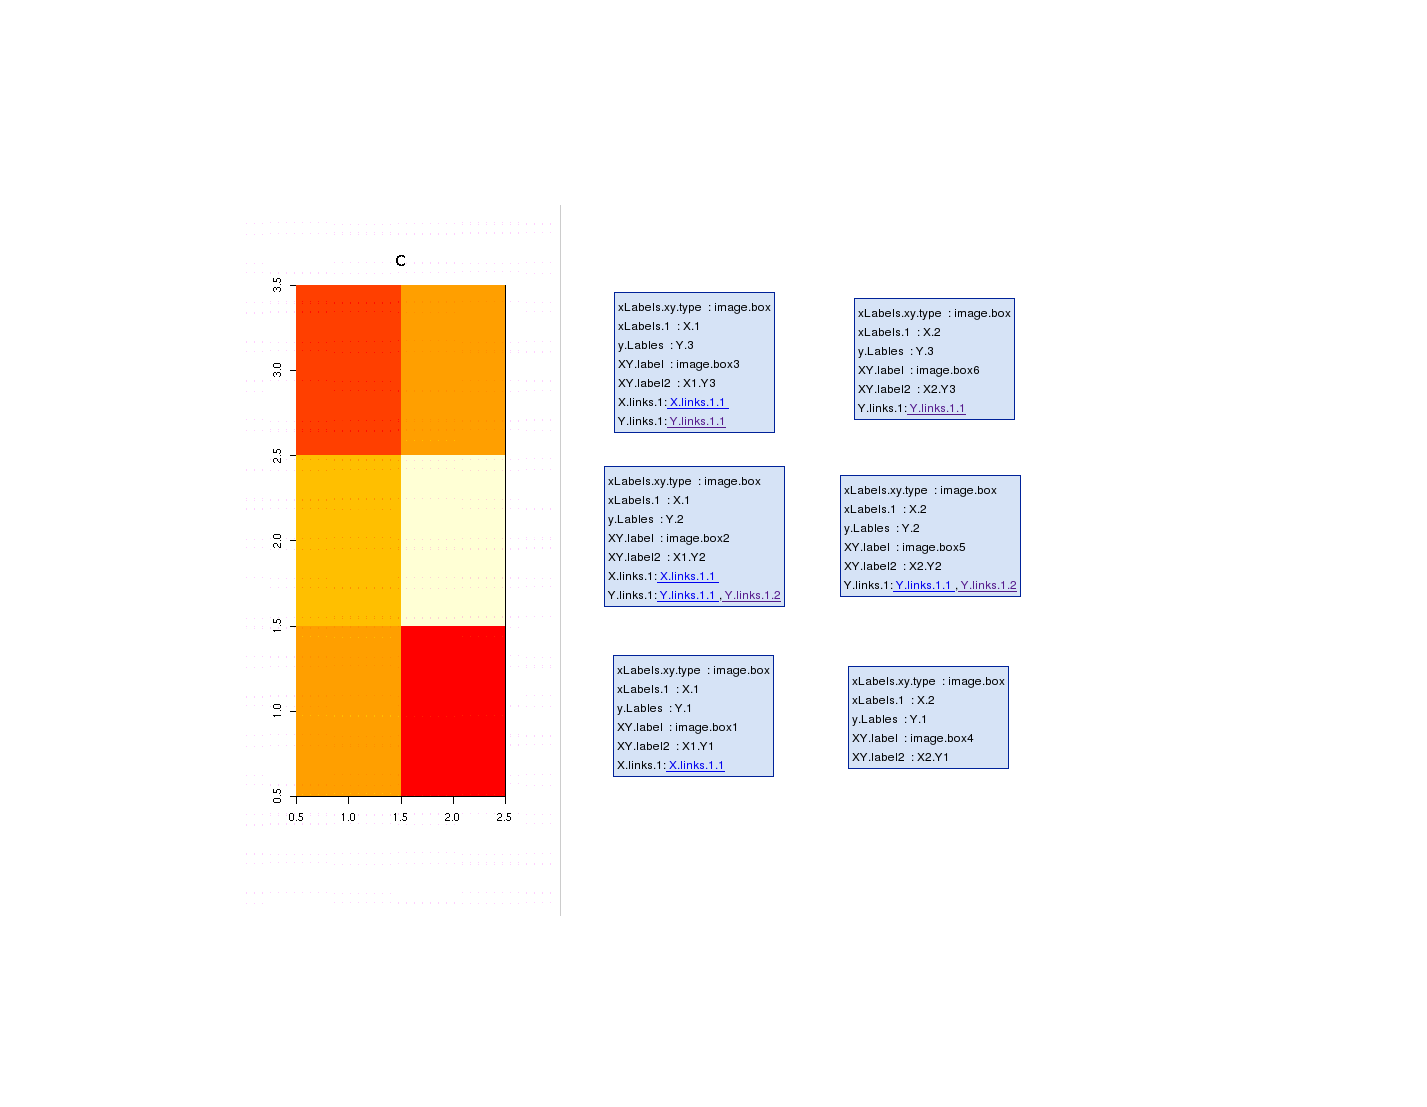
\includegraphics{imageToolTip}
\caption{Image figure with corresponding tool-tip display boxes}
\end{figure}
\end{center}



\vspace{5mm}

\large \indent {\bf{CREATING LAYOUT FIGURE 4}} 

\vspace{5mm}

\normalsize

Layout figure 4 will be a static or decoration plot only. No interactive data sets added. 


\subsection{makeSplot: Making the Plot}

\indent At any point after the Splot object is made, a plot can be generated for the object. If makeImap has not been utilized a static plot is created. If makeImap has been utilized, an interactive html file may also be generated. The following is an example call:

\begin{verbatim}

makeSplot(Splot,
          fname.root="Splot",
          dir="./",
          overwriteSourcePlot = NA,
          makeInteractive=TRUE,
          overrideInteractive=NA,
          Default=TRUE,
          header="v3",
          window.size = "800x1100", 
          returnObj = FALSE,
          getLims=FALSE)
\end{verbatim}

The following gives brief descriptions of the arguments, some will be discussed further in this section:

\begin{description}
\item{Splot:~}{an Splot, sendplot, object: see section on initSplot}
\item{fname.root:~}{character, base name to use for file[s] created}
\item{dir:~}{character, directory path for where the file[s] should be created}
\item{overwriteSourcePlot:~}{character, the type of file created: postscript, png, or jpeg}
\item{makeInteractive:~}{logical indicating if the interactive html file should be produced}
\item{overrideInteractive:~}{logical vector equal to the length of the number of figures in the layout, determines which interactive data should be included in the html file}
\item{Default:~}{logical, if a default region is set should it be included in the html file}
\item{header:~}{may either be v1,v2, or v3. This determines which tooltip header will be in the html file}
\item{window.size:~}{size of the html window. Only effective when header=v3}
\item{returnObj:~}{logical, indicates if the Splot object should be returned with updated information}
\item{getLims:~}{Used internally to get x and y limits of all figures. User does not need this argument.}
\end{description}

\indent In the automatic mapping portion of this function, .png (or .jpeg) and .tif files are created. The fname.root argument gives the base name for all these files to ensure that previously generated files are not accidentally overwritten. The dir argument is added as a prefix to the fname.root to create a full path name for the files generated. This will also be the name of the html file that is created if makeInteractive is TRUE. A static image may be generated without creating the html file by setting makeInteractive to FALSE. If makeInteractive is TRUE the application will attempt to make an interactive html. The files created are determined by the source.plot setting when the Splot object was created. If the user so chooses, they may override what is set in the Splot object by setting overwriteSourcePlot. If overwriteSourcePlot is NA, it uses the Splot object value. The options for overwriteSourcePlot are:  "ps" for postscript, "png" for a portable network graphics, or "jpeg" for a joint photographic experts group. \newline

\indent Tool-tip data must have been added through the makeImap function for each of the desired interactive figures. There may be occasions where information is added but it is not necessary to display in the html file. The argument overrideInteractive is a logical vector of length equal to the number of figures in the layout. It indicates if the figure's interactive data, if applicable, should be included in the html. If overrideInteractive is NA, it will use the default settings provided when initializing the Splot object. A default interactive region, which will be active everywhere in the figure that does not have an alternate setting through makeImap, may or may not be displayed through the argument Default. For more information on default region and how to set this region in the Splot object see section 5.1. The Default argument is therefore a logical TRUE if displayed, FALSE if hidden (only applicable if default has been set for Splot object). \newline

\indent The arguments header and window.size refer to qualities when viewing the html file. The header controls which header information is included for the html file. It also contains the needed javascript tooltip information necessary for interactive plots. The different versions of headers have different features or work on different web browsers. The main difference between the currently available headers are given below:

\begin{description}
\item{v1:~}{works well with Firefox and displays information in the upper right corner of the web browser}
\item{v2:~}{works well with Firefox and internet explorer and displays information at the mouse location}
\item{v3:~}{is the same as v2 except it allows control of the html window size. The default window size is 800x1100 and can be changed with the argument window.size}
\end{description}

\indent As mentioned in the v3 header description, if using that option the html window size may be adjusted for better viewing. The window.size argument defaults to "800x1100". It may be adjusted by entering a character value "<width> x <height>". The separation between the width and height must be "x". The size is in pixels. \newline

\indent {\bf{Note:}} The above description mentions Firefox and internet explorer for web browsers. These are the browser we have tested. Other collaborators have used different browser, the requirement for viewing is the browser must have javascript capabilities. Also note, depending on the browser, privacy settings may have to be altered to allow for interactive data to display. Browsers may block the interactive content as privacy risks or they are considered pop-ups.  \newline

The following is an example Splot call to make the interactive version of figure 7 :



\begin{verbatim}
Splot = makeSplot(Splot, fname.root="sendPlotEx", returnObj=TRUE)
\end{verbatim}




\subsection{Extra Functions}

\indent There are two other functions worth mentioning that will be described further:

\begin{description}
\item{addDefault:~}{adds a default region to interactive html}
\item{removeImap:~}{removes any or all sets of interactive mapping data for a given figure, or a default region}
\end{description}

\subsubsection{addDefault: Add Default Tool-tip Region}

A default region may be added in the html image map. A default region will span the entire layout of figures where other regions have not already been defined. The following is example code that will set a default region for an Splot object:

\begin{verbatim}
addDefault(Splot,
           data=NA,
           data.labels=NA,
           links=NA,
           links.labels=NA,
           asLink=NA,
           font.type="Helvetica",    
           font.color="black",  
           font.size="12",      
           bg.color='#D6E3F6',  
           returnVl=TRUE,
           saveFlag=FALSE,
           saveName="Splot.RData")
\end{verbatim}

\indent The data displayed in the tool-tip is controlled with the following arguments:
\begin{description}
\item{data:~}{character vector of all data to be displayed}
\item{data.labels:~}{character vector of labels corresponding to location in data}
\item{links:~}{character vector with complete web address}
\item{links.labels:~}{character vector of labels corresponding to location in links}
\end{description}

\indent The data and links arguments are different than in the makeImap function in that they are not matrix or data.frames. They are simply character vectors. The corresponding labels arguments, therefore, hold the names to use for labels in the tool-tip (since before column names from the data.frames are used). The argument asLink will be a single character vector with the complete web address or NA if no hyperlink is desired. Only one default region may be set at any given time.\newline

\indent The arguments for controlling the tool-tip display are the same as the makeImap section. Please refer to section 5.3 for more information on font.type, font.color, font.size and bg.color. \newline

\indent A new object is added to the Splot object to hold the default region information. The arguments returnVl and saveFlag therefore indicate if the new object should be returned or saved to a file. \newline

\indent As mentioned in section 5.4, a default region may be set but not displayed. If the addDefault function is run and the default information is saved in the Splot object, there is still the option when creating the html if the default tool-tip should be displayed. This is controlled through the makeSplot Default argument. See section 5.4 for more details. \newline

\indent The following will add a default tool-tip region to figure 7: 





\begin{verbatim}
Splot = addDefault(Splot, 
                   data=c("", "quick", "convenient", "highly customizable", 
                         "This is a default region",
                         "arial", "gray", "yellow" ), 
                   data.labels=c("Sendplot selling points", "   1", "   2", "   3", 
                         "type",
                         "tooltip.font", "tooltip.backgroundColor","tooltip.fontColor"),                    
                   links=c("http://www.buffalo.edu", 
                           "http://www.bioinformatics.buffalo.edu/"), 
                   links.labels=c("UB", "CoE"),
                   font.size=10, font.type="arial",
                   bg.color="gray", font.color="yellow")
\end{verbatim}


Note: The default region will only display if the makeSplot function is run with Default=TRUE:


\begin{verbatim}
Splot = makeSplot(Splot, fname.root="sendPlotEx", returnObj=TRUE, Default=TRUE)
\end{verbatim}

The above code make the tool-tip seen in figure 22.

\begin{center}
\begin{figure}

\includegraphics[width=1.8in, height=1.6in]{DefaultToolTip}
\caption{Example tool-tip default}
\end{figure}
\end{center}


\subsubsection{removeImap: Removing Interactive Regions}

\indent Sections 5.3 and 5.5.1 addressed adding sets of data for the tool-tip functionality. It is also possible to remove any set of data for a given figure or a set default region. This is achieved through the removeImap function:

\begin{verbatim}
removeImap(Splot,
           figure,
           subset=NA,
           returnVl=TRUE,
           saveFlag=FALSE,
           saveName="Splot.RData")
\end{verbatim}

\indent The arguments figure and subset control what set[s] of data is removed. 

\begin{description}
\item{figure:~}{Either a single numeric value corresponding to the figure as specified in the layout matrix or "Default"}
\item{subset:~}{Numeric indication of which set[s] of data to remove. Set numbers correspond to the order in which they were added (using makeImap)}
\end{description}

\indent To remove a set default region, the figure value should be "Default". If a default region was set it will be removed. It is only possible to remove data sets for a single figure at a time. The figure number corresponds to the plot region in the layout matrix. The subset argument controls what sets[s] for the given figure will be removed. If subset is left as NA, all the data for the figure will be removed. A numeric vector is the other option for the subset argument. The numbers will indicate which set[s] to remove. The set numbers correspond to the order in which they were added (by makeImap). The function will check to see if there are appropriate sets and remove all those that apply. \newline
\indent This function changes the Splot object. It is therefore necessary to specify if the new object should be returned or saved through the returnVl or saveFlag arguments. \newline
\indent The follow is an example removing the Default region:


\begin{verbatim}
Splot = removeImap(Splot, figure="Default", returnVl=TRUE, saveFlag=FALSE)
\end{verbatim}


\indent Going back to the example, there are three iMap regions for Figure 2: the blue points, the red points, and the polygon. The following will remove the interactive data for the red points: 



\begin{verbatim}
Splot = removeImap(Splot, figure=2, subset=2, returnVl=TRUE, saveFlag=FALSE)
\end{verbatim}

Notice how the figure specified is 2 and since the red points were the second data set added the subset is also 2. To remove all iMaps for a figure, leave subset as NA. The following removes all iMaps for the first figure:




\begin{verbatim}
Splot = removeImap(Splot, figure=1, subset=NA, returnVl=TRUE, saveFlag=FALSE)
\end{verbatim}


\section{closing remarks}


Look for our aCGH bioinformatics wrapper coming soon!

\end{document}

